%%%%%%%%%%%%%%%%%%%%%%%%%%%%%%%%%%%%%%%%%%%%%%%%%%%%%%%%%%%%%%%%%%%%%%%%%%%%%%%%
%2345678901234567890123456789012345678901234567890123456789012345678901234567890
%        1         2         3         4         5         6         7         8


\documentclass[letterpaper, 10 pt, conference]{ieeeconf}  % Comment this line out
                                                          % if you need a4paper
%\documentclass[a4paper, 10pt, conference]{ieeeconf}      % Use this line for a4
                                                          % paper

\IEEEoverridecommandlockouts                              % This command is only
                                                          % needed if you want to
                                                          % use theplp \thanks command
\overrideIEEEmargins
% See the \addtolength command later in the file to balance the column lengths
% on the last page of the document



% The following packages can be found on http:\\www.ctan.org
\usepackage{graphics} % for pdf, bitmapped graphics files
\usepackage{epsfig} % for postscript graphics files
\usepackage{mathptmx} % assumes new font selection scheme installed
\usepackage{times} % assumes new font selection scheme installed
\usepackage{amsmath} % assumes amsmath package installed
\usepackage{amssymb}  % assumes amsmath package installed
\usepackage{mathtools}
\usepackage[noadjust]{cite}
\usepackage{dblfloatfix}
\usepackage{color}
\usepackage{booktabs,tabularx}
\usepackage{optidef}

\renewcommand{\thefigure}{\arabic{figure}}

\title{\LARGE \bf
Fabric Soft Poly-Limbs for Physical Assistance of Daily Living Tasks  
}

%\author{ \parbox{3 in}{\centering Huibert Kwakernaak*
%         \thanks{*Use the $\backslash$thanks command to put information here}\\
%         Faculty of Electrical Engineering, Mathematics and Computer Science\\
%         University of Twente\\
%         7500 AE Enschede, The Netherlands\\
%         {\tt\small h.kwakernaak@autsubmit.com}}
%         \hspace*{ 0.5 in}
%         \parbox{3 in}{ \centering Pradeep Misra**
%         \thanks{**The footnote marks may be inserted manually}\\
%        Department of Electrical Engineering \\
%         Wright State University\\\textbf
%         Dayton, OH 45435, USA\\
%         {\tt\small pmisra@cs.wright.edu}}
%}

\author{Pham H. Nguyen, \textit{Student Member, IEEE}, Imran I. B. Mohd, Curtis Sparks, Francisco L. Arellano,\\ and Panagiotis Polygerinos$^{*}$, \textit{Member, IEEE}% <-this % stops a space
%\thanks{*Equally Contributing 1st Authors}% <-this % stops a space
\thanks{$*$ Corresponding Author}% <-this % stops a space
\thanks{Pham H. Nguyen, Curtis Sparks, and Panagiotis Polygerinos are with the Polytechnic School, Ira A. Fulton Schools of Engineering, Arizona State University, Mesa, AZ 85212, USA. 
         {\tt\small nhpham2@asu.edu; cmspark1@asu.edu; polygerinos@asu.edu}}%
\thanks{Imran I. B. Mohd The School for Engineering of Matter, Transport and Energy, Ira A. Fulton Schools of Engineering, Arizona State University, Tempe, AZ 85281, USA.
        {\tt\small imohd@asu.edu}}%
\thanks{Francisco L. Arellano The School of Biological Health Systems Engineering, Ira A. Fulton Schools of Engineering, Arizona State University, Tempe, AZ 85281, USA.
        {\tt\small flopezar@asu.edu}}%
}



\begin{document}



\maketitle
\thispagestyle{empty}
\pagestyle{empty}


%%%%%%%%%%%%%%%%%%%%%%%%%%%%%%%%%%%%%%%%%%%%%%%%%%%%%%%%%%%%%%%%%%%%%%%%%%%%%%%%
\begin{abstract}

This paper presents the novel design and development of a highly articulated, continuum, wearable, fabric-based Soft Poly-Limb (fSPL). The soft arm acts as an additional limb that provides compliant and safe mobile manipulation assistance to users with upper extremity impairments. In this work, a set of systematic design rules is presented for the creation of highly compliant soft robotic limbs through an understanding of their component’s behavior as a function of input pressure. These design rules are obtained by investigating a range of geometrical parameters of the f3CBAs through computational finite-element method (FEM) models focusing on the fSPL's articulation capabilities and payload capacity in 3D space. The motion and payload outputs of the fSPL and its components is investigated through experimental validations of the FEM models and preliminary evaluations of its capability to safely operate and interact with the wearer. Spatial mobility tests and pick-and-place experiments are demonstrated, while attached to a soft-waist belt that can comfortably store the fully collapsible fSPL when not in use.

\end{abstract}

%%%%%%%%%%%%%%%%%%%%%%%%%%%%%%%%%%%%%%%%%%%%%%%%%%%%%%%%%%%%%%%%%%%%%%%%%%%%%%%%
\section{INTRODUCTION}

Cervical Spondylotic Myelopathy (CSM) is a degenerative condition that is caused by general wear and tear or injury to the cervical region of the spinal cord, affecting limb functions and limiting independence \cite{lubelski2016}. As a result, individuals with CSM syndrome typically experience difficulty performing motor tasks, such as activities of daily living (ADLs). This population could benefit from a soft wearable collaborative robotic device, such as the fabric-based, Soft-Poly Limb (fSPL) presented in this work.

\begin{figure}[t!]
\centering
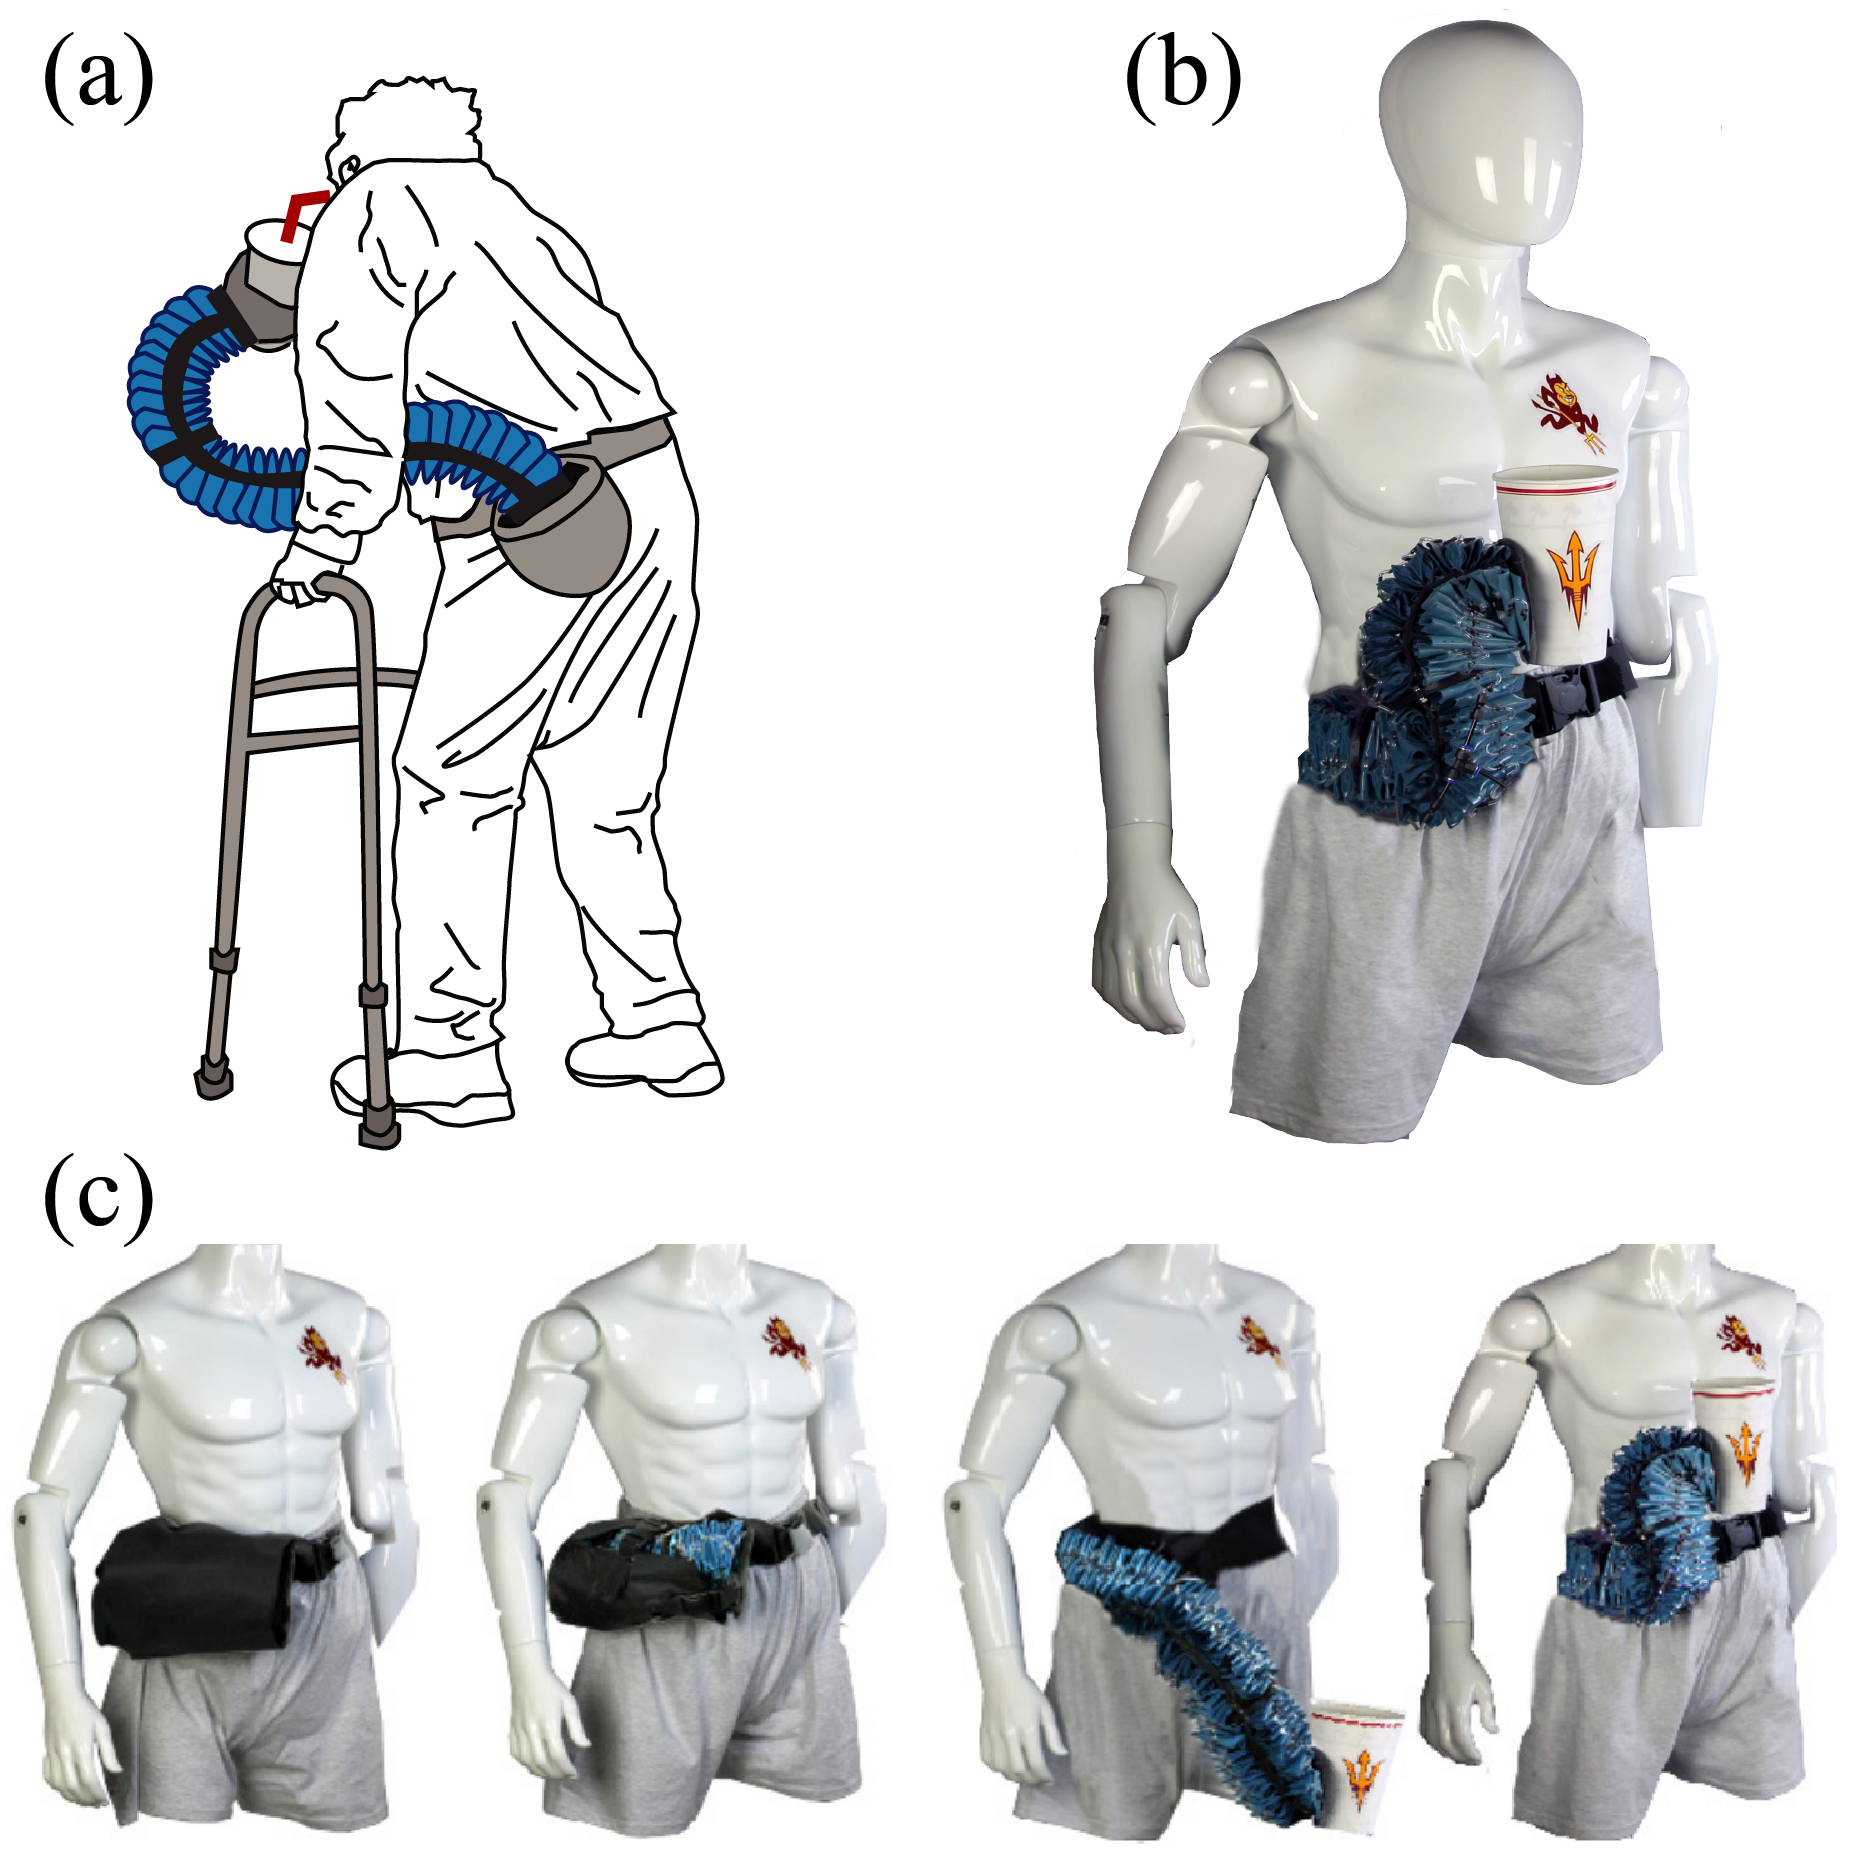
\includegraphics[width=0.45\textwidth]{Figures/fig1_new_v2}
\caption{ (a) Illustrated concept of the fabric-based Soft Poly Limb (fSPL). (b) The prototype fSPL mounted on a lightweight waist-belt system is a soft, lightweight, wearable robot that is designed to assist users with activities of daily living (ADL). (c) Left-to-right: the limb is collapsed and stored in a pouch and then deployed to assist with tasks, such as picking up a cup.}
\label{fig:fig1}
\vspace{-1.5em}
\end{figure}

Wearable robotics manipulators are devices that can be worn to provide an additional appendage to assist and support the user to perform tasks. These devices do not kinematically have to match the human body's anatomy, like exoskeletons \cite{gopura2011} or prosthetic devices \cite{bogue2009}. Therefore, they do not require extra consideration in terms of alignment with biological joints. Recent examples of different wearable collaborative robotic devices include robotic legs \cite{kurek2017,parietti2015}, arms \cite{parietti2014,saraiji2018,vatsal2017}, fingers \cite{hussain2017b,wu2015,tiziani2017}, ranging from the industrial \cite{parietti2014} and medical settings \cite{tiziani2017}. 

% The recent rise of wearable robotic manipulators have brought up questions of user controllability. The possibility of controlling an extra limb has been previously investigated and it is known that the human central nervous system (CNS) is found to be capable of learning to control additional limbs \cite{guterstam2011,tsakiris2010}. The controllability of robotic limbs has been explored in preliminary research, utilizing biological signals from the torso muscles \cite{parietti2017}, foot \cite{sasaki2017}, elbow \cite{wu2015}, and the forehead frontalis muscles \cite{salvietti2017}.

Wearable manipulators currently face limitations that originate from their rigid designs, like their weight, bulk, and the interaction between rigid elements and the human body \cite{delAma2012}. Soft robotics has emerged as one of the solutions to tackle the aforementioned challenges. The recent influx of soft robots have led to the introduction a variety of soft continuum manipulators made of a variety of soft actuators. The categories of soft continuum manipulators is subdivided based on the actuators that constitute them, including cable-driven \cite{mcMahan2005,calisti2011}, pneumatic artificial muscles (PAMs) \cite{walker2005,godage2016,yasmin2017,giannaccini2017}, elastomeric \cite{cianchetti2013,marchese2015,robertson2017,gong2018}, origami \cite{santoso2017}, and inflatable-fabric \cite{sanan2013,hawkes2017,ohta2017,best2016,liang2018,takeichi2017,kim2018,liang2017c} based manipulators. 
% * <polygerinos@asu.edu> 2018-09-09T23:28:36.896Z:
% 
% > The recent influx of soft robots have led to the introduction a variety of soft continuum manipulators made of a variety of soft actuators. The categories of soft continuum manipulators is subdivided based on the actuators that constitute them, including cable-driven \cite{mcMahan2005,calisti2011}, pneumatic artificial muscles (PAMs) 
% it would have been great to have your review paper cited here....if they accept we can add in january 
% 
% ^.

The fusion of soft robotics and wearable manipulators has created a new category of robotics which we call, Soft Poly-Limbs (SPLs). Limited research has started to emerge in this category, Tiziani et al. \cite{tiziani2017} has introduced a soft poly-finger device, Liang et al. \cite{liang2017c} have suggested a single DOF fabric-based soft poly-arm device that would eventually be integrated as a wearable robot, but have not evaluated the device for this use case yet. Finally, we recently introduced a safe, elastomeric, SPL device \textbf{cite[]} with nine degree-of-freedom, capable of lifting weights horizontally up to 1.4$x$ its own body weight and wrap around objects to lift approximately 4$x$ its own weight. 
% * <polygerinos@asu.edu> 2018-09-09T23:29:50.443Z:
% 
% > Soft Poly-Limbs (SPLs)
% cite your SORO  paper here
% 
% ^.

In this paper, we have designed a novel, highly-articulated, high-power-to-weight ratio, fabric-based, upper-limb SPL capable of assisting users with ADL tasks, as seen in Fig. 1. We provide a material study of various fabric materials tested to achieve the current design of the fabric-based SPL (fSPL). We further investigate the mechanical behavior of the fSPL and its components by using a varying set of design parameters to optimize the payload capacity of the fSPL by using computational finite element method (FEM) models that are also validated experimentally. Finally, through experimentation we showcase the potential of the novel fSPL to work safely around the wearer, display its high payload-to-weight ratio, and assist with ADLs . 


\section{Functional Requirements and Design of fSPL }
\label{sec:func_req}
\begin{table}[b!]
\caption{Requirements for a fabric-based Soft-Poly Limb (fSPL)} 
\label{tab:spec_table}
	\begin{tabularx}{0.48\textwidth}{*2l}    \toprule\toprule
	\textbf{\emph{Characteristics}} & \textbf{\emph{Requirements}} \\\midrule
	Weight of Device    & less than 1.0$kg$  \\ 
	Profile of fSPL & less than 100$mm$ diameter \\ 
	Payload (fully extended)    & Approx. 1$kg$  \\ 
	Payload (whole-body grasp) & 2$x$ the weight of device \\ 
	Max. Reach Length    & Length of male arm (0.59$m$)  \\ 
	Min. Retraction Length & Half of fully stretched SPL \\ 
	Safety    & Easy to don-and-doff \\ 
	 &Does not interfere with\\
     &biological limb's movement\\
	Degrees-of-Freedom (DOF) & At least 9DOF \\ 
	Degrees of Curvature of Each Segment & 180$^{\circ}$ \\\bottomrule
	 \hline
	\end{tabularx}
\end{table}

In order to provide long-term options to CSM patients who have loss/reduced function in their hands and arms we have laid out a soft robotic architecture with versatile specifications, as summarized in Table \ref{tab:spec_table}. We intend to provide the wearer with a highly deployable, full-length SPL that interacts safely with the user, and can be compressed to at least half of its original length and stowed away in a small pouch attached to a waist belt, without adding bulkiness, while still being extremely light weight (under 1.0$kg$). The SPL should be a highly maneuverable continuum manipulator with 9-DOFs, while being compliant and configurable. The system should also be able to carry up to approximately 1$kg$ of payload at its end-effector position when fully-extended and parallel to the ground and carry up to twice its body weight by wrapping around the object using a whole-body grasping method, that can only be offered through such soft continuum systems. 
% * <polygerinos@asu.edu> 2018-09-09T23:52:24.093Z:
% 
% > 1$kg$ of payload at its end-effector position when fully-extended and parallel to the ground and carry up to twice i
% you do not explain why 1kg and why twice the load...please add and break into smaller sentences 
% 
% ^.
% * <polygerinos@asu.edu> 2018-09-09T23:48:19.888Z:
% 
% > with 9-DOFs
% the 9dofs is highly arbitrary and you do not provide any good explanation.
% plus still you havent decided if continuum arms can claim degrees of freedom like rigid arms do. still i think here we have infinite/multiple dofs  that offer high actuation redundancy.
% 
% ^.

In order to achieve the functional requirements, we introduce the design of a fSPL made up of three modular segments. These segments are called fabric 3-chambered bending actuators (f3CBAs). Each segment further consists of three arrays with bending actuators arranged in an equilateral triangle fashion. The length of the SPL is designed to match the length of an average sized adult male arm, which is approximately 0.59$m$, from the tip of the shoulder to the center of the wrist.
% * <polygerinos@asu.edu> 2018-09-09T23:56:45.521Z:
% 
% > In order to achieve the functional requirements, we introduce the design of a fSPL made up of three modular segments. These segments are called fabric 3-chambered bending actuators (f3CBAs). Each segment further consists of three arrays with bending actuators arranged in an equilateral triangle fashion. The length of the SPL is designed to match the length of an average sized adult male arm, which is approximately 0.59$m$, from the tip of the shoulder to the center of the wrist.
% is there a figure that the reader can see to follow the components that comprise the arm?
% 
% ^.

Each bending actuator array is comprised of multiple high-strength, heat-sealed, TPU-coated nylon (200D) fabric actuators that are arranged and sewn onto a strain-limited fabric layer. The functionality of the bending actuator arrays have previously been highlighted in our previous work \cite{thalman2018} where thermoplastic polyurethane (TPU) actuators were encased in nylon fabric casings in order to withstand higher pressure and provide better outputs. In this paper, a variety of heat-sealable TPU-coated nylon fabric materials are explored to develop soft actuators that are robust to external environmental interactions, allow for a single-step fabrication process to save manufacturing time, and are capable of withstanding even higher pressures than before, thus achieving higher bending and torque outputs.
% * <polygerinos@asu.edu> 2018-09-09T23:59:17.511Z:
% 
% > Each bending actuator array is comprised of multiple high-strength, heat-sealed, TPU-coated nylon (200D) fabric actuators that are arranged and sewn onto a strain-limited fabric layer. 
% again, a reference to a figure could go a long way in visualizing into the reader's head what you mean.
% 
% ^.
% * <polygerinos@asu.edu> 2018-09-09T23:59:07.309Z:
%
% > Each bending actuator array is comprised of multiple high-strength, heat-sealed, TPU-coated nylon (200D) fabric actuators that are arranged and sewn onto a strain-limited fabric layer.
%
% ^.

The f3CBA segments of the fSPL and the actuators in the actuator arrays are designed to be interchangeable and easily replaceable for maintenance. When not pressurized, the fSPL can be compressed to more than half its full length allowing for ease of carriage. We designed the fSPL to be mountable on a comfortable waist belt system that weighs less than 0.5$kg$. This belt allows the integrated wearable limb to don-doff easily. The end-effector unit is also customizable for the specified task. The fSPL is also capable of utilizing its entire soft body to grasp and carry objects larger in size and weight, something that traditional rigid robotic arms are incapable of achieving. The pneumatic system is currently off-board and controlled by our experimental platform \cite{nguyen2018} to monitor and control the SPL.





% \begin{figure}[t]
% \centering
% 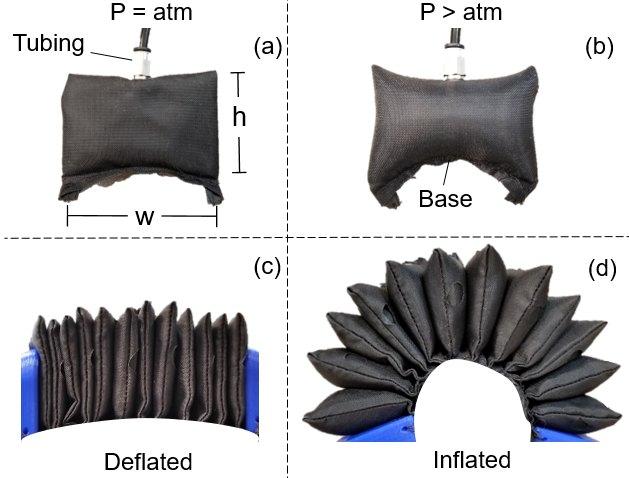
\includegraphics[width=0.4\textwidth]{V1_device.PNG}
% \caption{(a) Deflated soft actuator with labeled dimensions for width, $w$ and height, $h$. (b) Inflated soft actuator. (c) Deflated soft actuator array. (d) Inflated soft actuator array.
% }

% \label{fig:array}
% \end{figure}




% \begin{figure}
% \centering
% 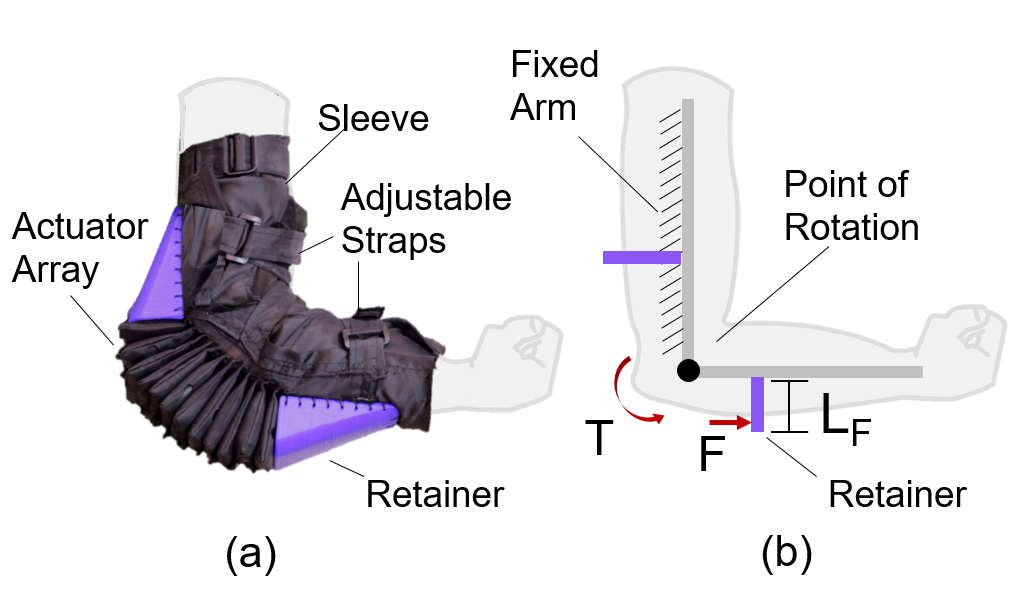
\includegraphics[width=0.45\textwidth]{arm.PNG}
% \caption{Final Design of the soft robotic elbow sleeve (left) and the governing free body diagram (FBD) of the actuator array against the elbow (right)}
% \label{fig:arm}
% \vspace{-1.5em}
% \end{figure}


\begin{figure*}[t!]
\centering

\includegraphics[width=1.0\textwidth]{Figures/load_and_optimization_v2}
\caption{Payload Capability compared between FEM and Experimentally Validated a) Actuator Array b) f3CBA segment c) FEM analysis of number of number of actuators and ratio (r) with regards to the force generated by bladder actuator array.}
\label{fig:opti_payload}
\section{\vspace{-1.5em}}
\end{figure*}

\begin{figure}[b!]
\centering
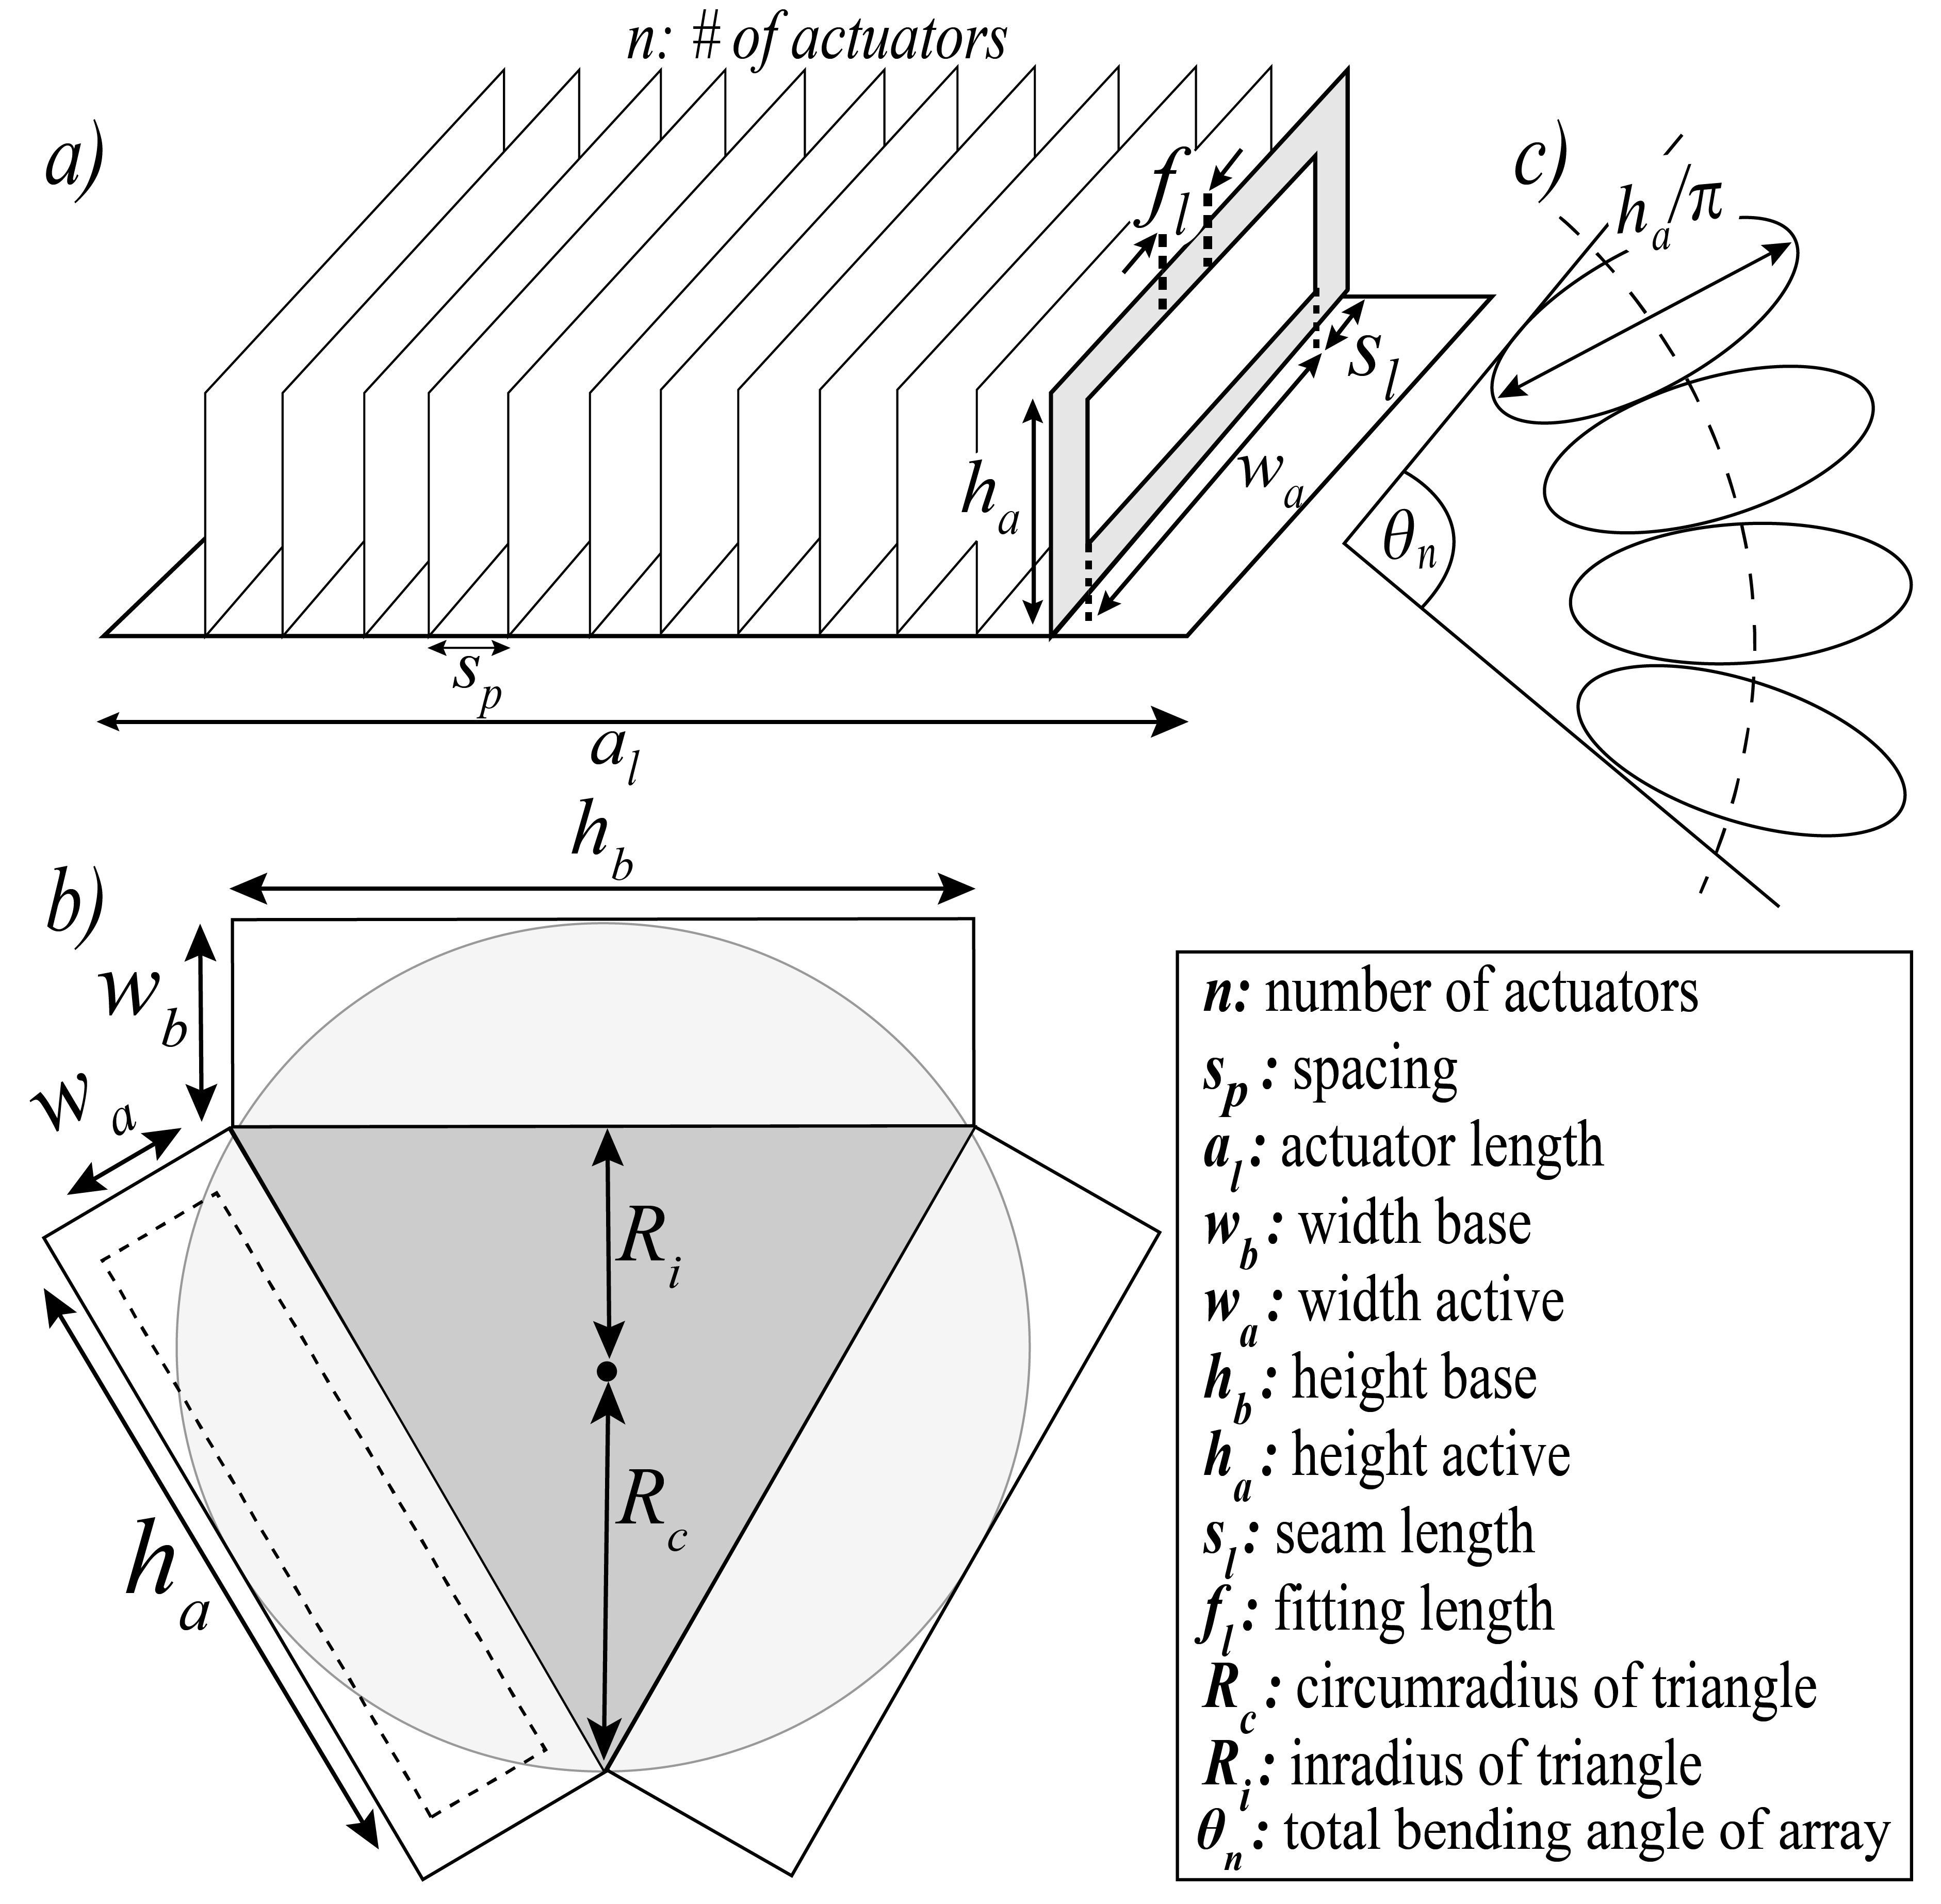
\includegraphics[width=0.45\textwidth]{Figures/geom_param_v5}
\caption{Geometrical Parameters of fSPL. a)Isometric view of bladder actuator array. b) Bottom view of f3CBA. c) Side view of bending bladder actuator array.}
\label{fig:geom_param}
\vspace{-1.5em}
\end{figure}



\section{ Materials and Characterization of fSPL} 

\subsection{Material Selection and Characterization}
\label{sec:mat_select}


\begin{table}[b!]
\caption{Material Properties of TPU Coated Nylon Fabrics} 
\label{tab:materialproperty_table}
	\begin{tabularx}{0.48\textwidth}{l|c|c|c}   \toprule\toprule
    \centering
    \small
    \setlength\tabcolsep{11pt}
	\textbf{\emph{Material}} & \textbf{\emph{Density (N) }} & \textbf{\emph{Seal Strength}} & \textbf{\emph{Burst }} \\[-1pt]
                             &                              & \textbf{\emph{(kg/m$^3$)}} & \textbf{\emph{Strength}}\\
                             &                              &                            & \textbf{\emph{(MPa)}}\\\midrule
	Rockywoods 200D &840.00 &168.35 & 0.53+5.821 \\
    Outdoor Oxford 200D  &757.58 &  183.68 & 0.48+4.518\\
    Ripstop 200D &758.62 & 192.19 & 0.4+2.466\\
    Seatle Diamond 200D &892.86 & 164.75 & 0.36+3.855\\
    DIY Packraft 400D & 982.46& 155.32 & x\\
    DIY Packraft 1000D &1000.00 & 236.17 & x\\
    Taffeta 70D &700.00& 142.13 & x\\\bottomrule 
    \hline
	\end{tabularx}
\end{table}

The extremely lightweight design of the fSPL with high payload capacity, is enabled by carefully testing a set of TPU-coated nylon fabrics with dernier values ranging from 70D to a 100D, (the dernier number indicates the fiber thickness of the filament used), as seen in Table \ref{tab:materialproperty_table}. 

We perform a seal strength peel test, following the ASTM F88/F88M-15. From these tests we select the top four materials demonstrating the highest seal strength and lowest densities %Although the seal strength for the DIY packraft 1000D material was the highest, it was deemed unviable because its incompressibility and density, which would affect the weight and retraction length of the fSPL. 
% * <polygerinos@asu.edu> 2018-09-10T00:13:51.898Z:
% 
% > %Although the seal strength for the DIY packraft 1000D material was the highest, it was deemed unviable because its incompressibility and density, which would affect the weight and retraction length of the fSPL. 
% this could be in discussion, although not super useful  and could be omitted entirely
% 
% ^.
and further test them for the maximum pressure they could withstand (burst test), using ASTM F2054. Based on the results, the Rockywoods 200D heat-sealable TPU-nylon fabric (Rockywoods Fabric, Loveland, CO) is chosen for its highest burst strength of 0.53$MPa$. Finally, the elastic Young's modulus for the selected material is determined using the ASTM D882 protocol and found to be 489.9$MPa$.

% Firstly, the individual bladders need to be able to maintain a tight seal under high stresses in order to remain airtight. The TPU seal strength for each material is tested using the ASTM F88/F88M-15 standard which involves applying axial tensile stress on the seal of the TPU-coated nylon fabrics. The test for each material was conducted 3 times and the average maximum seal strength values were calculated and tabulated as seen in Table \ref{tab:materialproperty_table}. The materials with the highest seal strength were proceeded for further testing. Although the seal strength for the DIY packraft 1000D material was the highest, it was deemed unviable because its incompressibility and density, which would affect the weight and retraction length of the fSPL.  

% The chosen materials were tested for their maximum burst strength using ASTM F2054. Three tests were conducted for each material and the average maximum pressure value was recorded in Table \ref{tab:materialproperty_table}. Based on the results, the Rockywoods 200D heat-sealable TPU-nylon fabric (Rockywoods Fabric, Loveland, CO) was chosen for its highest burst strength of 0.53$MPa$.

% Finally, the elastic modulus for the selected material is determined using ASTM D882, where axial tensile stress is applied to a fabric piece with measurements of 0.26x0.00254$m$ with a rate of 25$mm/min$ until failure. The calculated Young’s Modulus of Rockywoods 200D is calculated to be 498.9 $MPa$.



% \subsection{Geometrical Parameters}





% \begin{figure}[t!]
% \centering
% 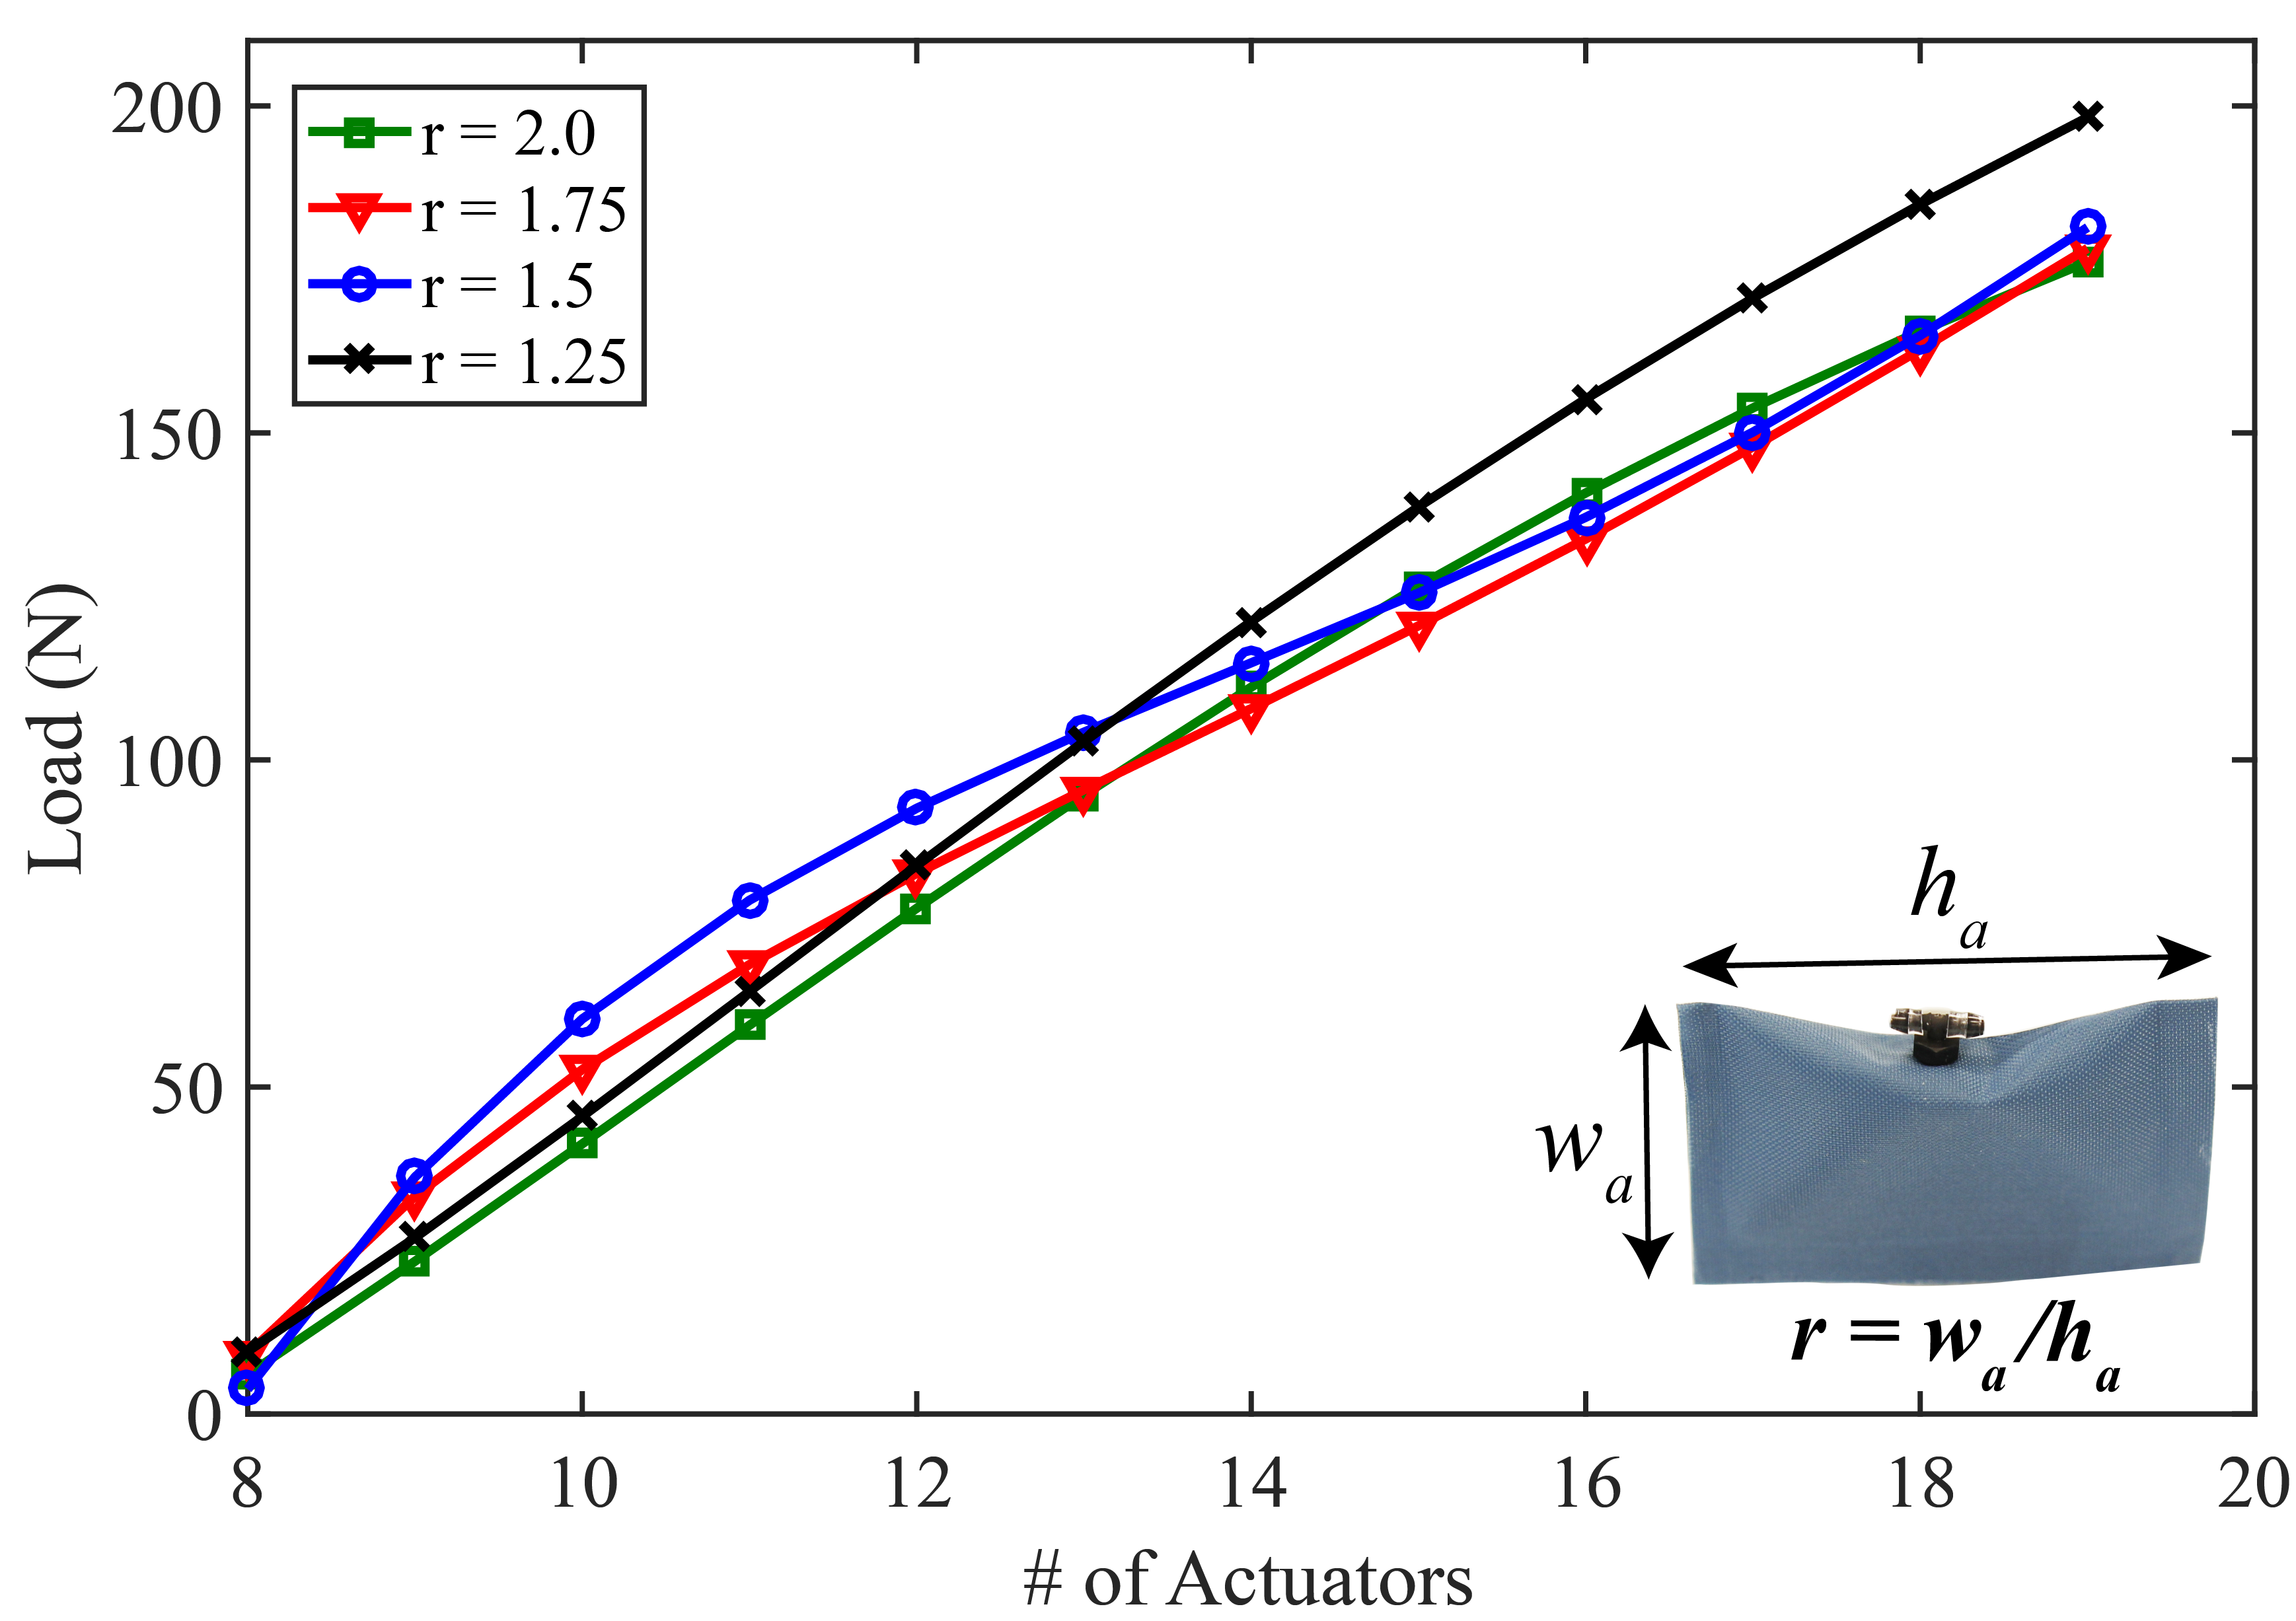
\includegraphics[width=0.48\textwidth]{Figures/fem_opti_v4}
% \caption{FEM analysis of number of number of actuators and ratio (r) with regards to the force generated by bladder actuator array.}
% \label{fig:fem_opti}
% \vspace{-1.5em}
% \end{figure}

% To study the payload and bending quality of the fSPL, a set of geometrical parameters highlighted in Fig. \ref{fig:geom_param} are studied. Figure \ref{fig:geom_param}a) depicts the isometric view of a single  actuator array of length $a_{l}$, consisted of $n$ number of actuators spaced at $s_{p}$. Each actuator is consisted of 4 main geometrical parameters, the fitting length ($f_{l}$), the seal length ($s_{l}$), the active width ($w_{a}$) and height ($h_{a}$). When the actuators are inflated, it is assumed to take a circular shape and therefore the active height, $h_{a}$, becomes $\frac{h_a}{\pi}$ and all the interacting actuators create a combined bending angle of $\theta_{n}$ as seen in Fig. \ref{fig:geom_param}b). 

% Figure \ref{fig:geom_param}c) shows the view of the base of a single f3CBA, where three  actuator arrays are arranged in an equilateral triangle fashion. The parameters include the circumradius of the equilateral triangle($R_{c}$), the inradius of the equilateral triangle ($R_{i}$), the width of the actuator ($w_{b}$), the height of the actuator ($h_{b}$), the active width of the actuator ($w_{a}$), and the active height of the actuator ($h_{a}$). 


\subsection{Geometrical Parameters of Bladder }
% * <polygerinos@asu.edu> 2018-09-10T00:18:39.923Z:
% 
% > Bladder 
% be consistent with the names you use...this is the first you call something a bladder. please revise
% 
% ^.
To study the payload and bending capabilities of the fSPL prior to fabrication, a set of geometrical parameters, as highlighted in Fig. \ref{fig:geom_param}, are studied. The three main geometrical parameters studied and optimized are the active width and height of the actuators ($w_{a}$ and $h_{a}$), and the number of actuators ($n$) based on their major contribution to the bending and payload capacity of the fSPL.

The active height ($h_{a}$) contributes to the bending capability, while the active width ($w_{a}$) contributes to the stability to the actuator array. If $w_{a}$ is less than $h_{a}$ then the contact surface between consecutive actuators will be small and therefore the actuators will slip resulting in torsion effects and incorrect distribution of force from actuator to actuator.

Therefore, $w_a$ is set to be greater than $h_a$ by a ratio $r$ that is larger that $1.0$. The active width and height are also constrained by the diameter of the physical tube fitting $f_l$ that will be used, which is 6.23$mm$, and the heat seam width $s_l$ created by the heat sealer, which is 5$mm$. The spacing between the actuators ($s_{p}$) is limited to above $7.5mm$ because of sewing manufacturing limitations. Both the active width and height of the actuator are also constrained by $R_{c}$, which also defines the cross-sectional radius of the fSPL, constrained to 50$mm$. The $\theta_{n}$, or the angle of the inflated  actuator array, is designed to achieve at least 180$^{\circ}$ when fully inflated. The physical constraints mentioned above are seen as follows:
% * <polygerinos@asu.edu> 2018-09-10T00:21:43.743Z:
% 
% > is larger that $1.0$.
% if you add another curve in fig. 2c with value smaller than 1.0 do not forget to change this too
% 
% ^.


\begin{align*}
R_c &= 50mm,    &  s_l &\geq 5mm,      &  \theta_n&=180^\circ,\\
f_l&=6.23mm,         &  a_l&=160mm,   &  s_p&\geq7.5mm.
\label{eq:constraints}
\end{align*}

Using the number of bladders ($n$), the spacing ($s_{p}$) and the active height ($h_{a}$) can be calculated as follows:
% * <polygerinos@asu.edu> 2018-09-10T00:27:02.256Z:
% 
% > bladders 
% again the word bladders..
% 
% ^.
\begin{align} 
w_a &= r\cdot h_a \\
s_p &=  \frac{(a_{l} - 2\cdot(a_l/n))}{n} \\ 
h_a &=  \frac{s_p \cdot \pi}{2\cdot(1-sin(\theta_n/(2\cdot n))} \label{eq:wa_sp_ha}
\end{align}

From the circumradius ($R_c$) and inradius ($R_i$) of Fig. \ref{fig:geom_param}b, we can calculate the active width ($w_a$) as follows:
\begin{align} 
w_a &\leq  R_c/(\frac{\sqrt{3}}{6} + \frac{1}{r}) - 2\cdot s_l -f_l \label{eq:wa_ha}
\end{align}

\subsubsection{FEM Optimization of Geometrical Parameters}

% \begin{figure}[b!]
% \centering
% 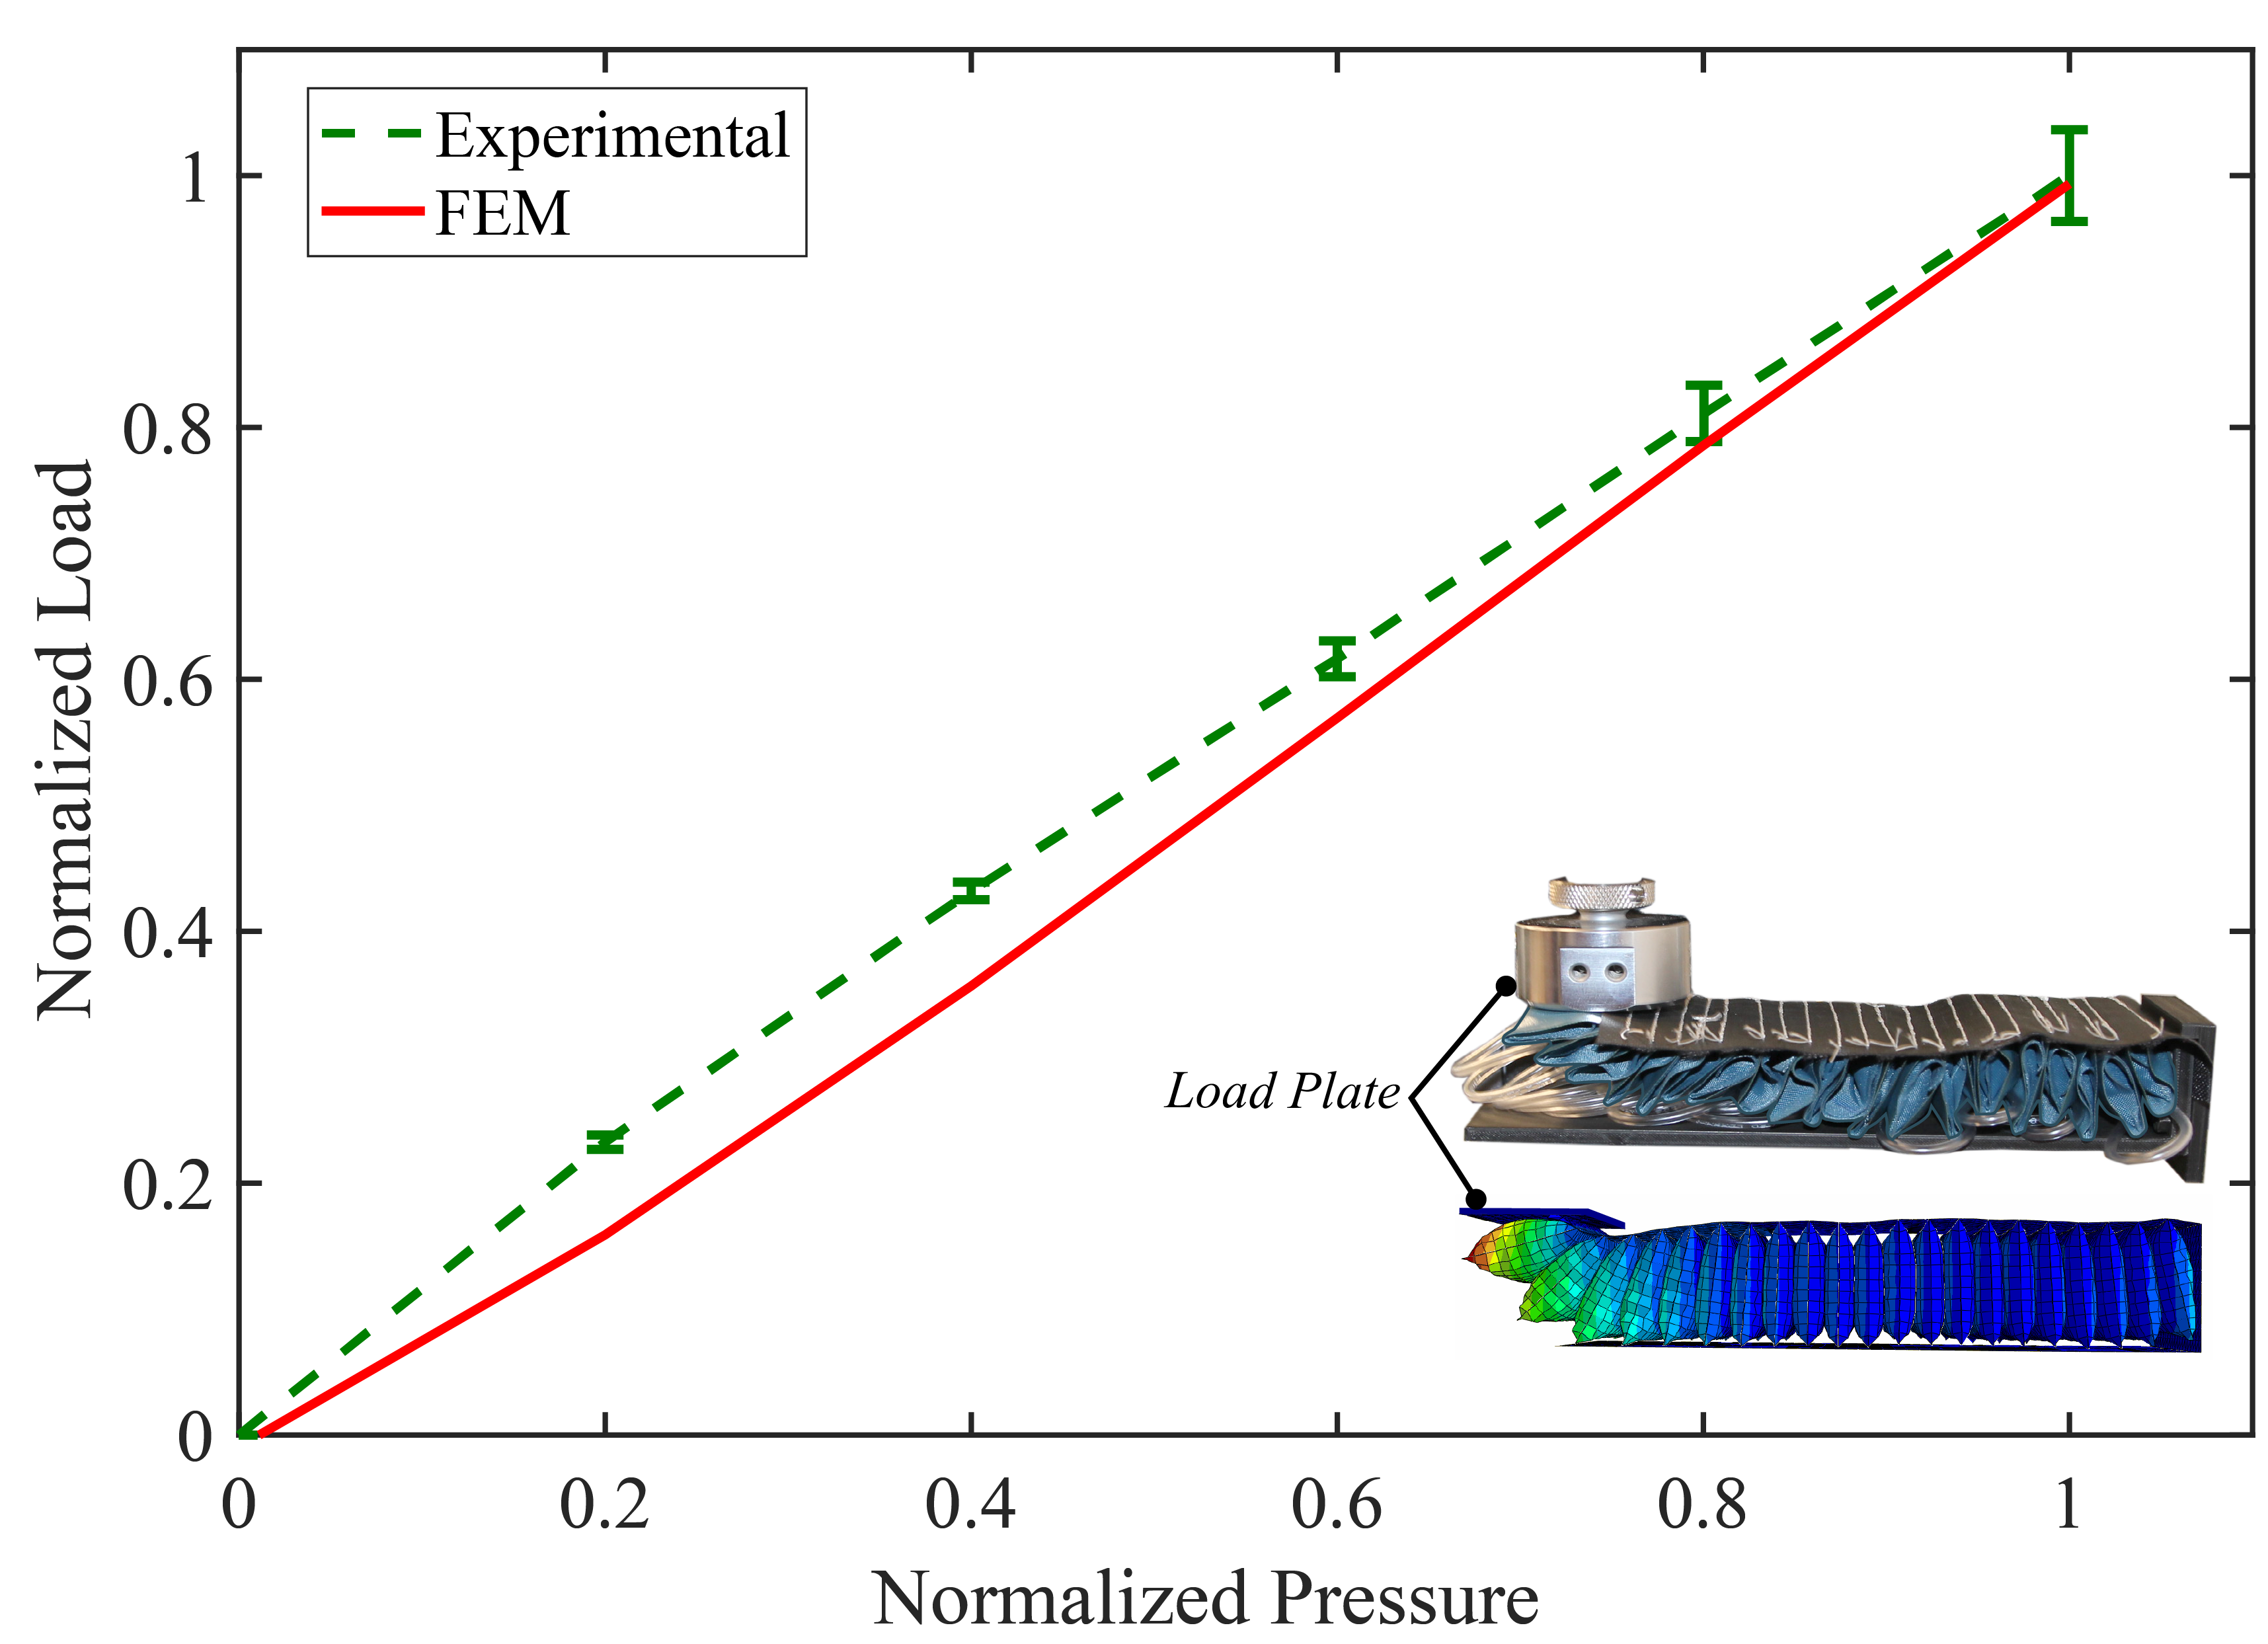
\includegraphics[width=0.45\textwidth]{Figures/single_FEM_REAL}
% \caption{Payload Capability of a Single Bladder Array compared between FEM and Experimentally Validated}
% \label{fig:single_fem_real}
% \vspace{-1.5em}
% * <polygerinos@asu.edu> 2018-09-10T01:20:49.833Z:
% 
% > % \label{fig:single_fem_real}
% > % \vspace{-1.5em}
% 
% all good but you have forgotten to add a critical explanatory paragraph that speaks of how you made the FEM model....explicit, shells, element types...interactions...etc
% 
% ^.
% \end{figure}

An optimization function is used that attempts to maximize the tip force of a bending actuator array as seen in Fig. \ref{fig:opti_payload}c). This tip force is simulated using computational FEM model simulations with two varying parameters, the ratio ($r$) and the number of actuators ($n$). We start by varying the ratio ($r$) from $1.25$ to $2.0$, as seen in Fig. \ref{fig:opti_payload}c. We use these ratios $r$ to calculate $w_a$ and $h_a$ through Eq. 2 and 3. Finally, the number of actuators ($n$) is varied based on the minimum and maximum $s_p$. The maximum $n$ is determined from Eq. 2 by the minimum $s_p \geq 7.5mm$, which demonstrates that $n = 19$ is the optimum number.  The minimum $n$ is determined by the number of actuators required to generate significant tip force from the actuator array, this is determined with FEM simulations as $n = 8$. As seen in Fig. \ref{fig:opti_payload}c, adding more actuators in the array contributes to a higher tip force. By varying the ratio ($r$) between $w_a$ and $h_a$, we notice a fairly similar trend across most of the explored ratios . Therefore, the configuration that is less likely to present actuator slippage when pressurized, which could present torsion effects of the overall limb, is selected, with $r =2.0$. Finally, in order to obtain a configuration that produces the highest amount force, the maximum $n$ possible ($n = 19$) in terms of fabrication restrictions is chosen. The FEM model is experimentally validated in Section~\ref{sec:act_array_fem_real}
% * <polygerinos@asu.edu> 2018-09-10T00:39:38.877Z:
% 
% > $r$
% sometimes r is in () sometimes not...be consistent
% 
% ^.
% * <polygerinos@asu.edu> 2018-09-10T00:38:42.639Z:
% 
% > This tip force is simulated using computational FEM model simulations with two varying parameters, the ratio ($r$) and the number of actuators ($n$). We start by varying the ratio ($r$) from $1.25$ to $2.0$, as seen in Fig. \ref{fig:opti_payload}c). We use these ratios $r$ to calculate $w_a$ and $h_a$ through Eq. 2 and 3. Finally, the number of actuators ($n$) is varied based on the minimum and maximum $s_p$. The maximum $n$ is determined from Eq. 2 by the minimum $s_p \geq 7.5mm$, which demonstrates that $n = 19$ is the optimum number.  The minimum $n$ is determined by the number of actuators required to generate significant tip force from the actuator array, this is determined with FEM simulations as $n = 8$. As seen in Fig. \ref{
% please revise...very confusing..
% 
% ^.
% * <polygerinos@asu.edu> 2018-09-10T00:34:45.036Z:
% 
% > s seen in Fig. \ref{fig:opti_payload}c).
% where is this seen in that figure??
% 
% ^.
% * <polygerinos@asu.edu> 2018-09-10T00:32:07.439Z:
% 
% > An optimization function is set
% what optimization function exactly? where is it?
% 
% ^.
% * <polygerinos@asu.edu> 2018-09-10T00:28:54.013Z:
% 
% >  seen in Fig. \ref{fig:opti_payload}c)
% make sure your figures are in the correct order...
% 
% ^.


\begin{figure}[t!]
\centering
\includegraphics[width=0.5\textwidth]{Figures/fabrication}
\caption{Fabrication of the fSPL. a) The bladder array when inflated. b) The CNC Process to fabricate bladders. c) Each singular bladder. d) The entire fSPL composed of 3 segments of f3CBAs.}
\label{fig:fabrication}
\vspace{-1.5em}
\end{figure}

\section{fSPL Manufacturing and Integration}


The fabrication process of the fSPL shown in Fig. \ref{fig:fabrication} begins with the creations of fabric TPU-coated nylon fabric actuators (6607, Rockywoods Fabric, CO). The material is cut into shape using a laser cutter (Glowforge Pro, Glowforge, Seattle, WA) and the pneumatic fittings are attached (5463K361, McMaster-Carr, Elmhurst, IL). A sealant is also added around the pneumatic fittings to prevent air leakage (Seam Grip, Gear Aid, Bellingham, WA). The material with the fittings are arranged on a customized CNC router (Shapeoko 3, Carbide Motion, Torrance, CA) with a soldering iron tip set at 232$^{\circ}$C and traced to seal the fabric bladders, as seen in Fig. \ref{fig:fabrication}b. This apparatus enables rapid heat-sealing of a variety of fabric soft actuator patterns of different shapes and materials accurately and repeatedly, up to 25 individual actuators at a time for this limb design. Fabric pockets for the individual actuators are then evenly sewn into an array configuration as seen in Fig. \ref{fig:fabrication}a), using a sewing machine (Memory Craft 6500P, Janome, Hachioji, Tokyo). The individual actuators as depicted in Fig. \ref{fig:fabrication}c, are then inserted into the pockets to create an actuator array, as shown in Fig. \ref{fig:fabrication}a. This approach allows for ease of replacement of the actuators during maintenance. Three sets of 3 actuator arrays are then arranged and sewn into an equilateral triangle prism called the fabric 3-chambered bending actuators (f3CBAs) shown in Fig. \ref{fig:fabrication}d. Modular 3D-printed connectors are sewn into the distal and proximal ends of the f3CBAs and are used to connect each other together, creating the complete the fSPL in Fig. \ref{fig:fabrication}d. The modularity of the connector pieces also allows for the addition of a variety of end-effectors to be mounted at the tip of the fSPL such as a suction cup (5427A636, McMaster-Carr, Elmhurst, IL). A zippered fabric pouch is used to house the fSPL in a compressed state for ease of storage. To interface the fSPL with the human body, the fabric pouch is sewn onto a modified technical belt (S\&F Deluxe Technical Belt, Lowepro, Petaluma, CA) as shown in Fig. \ref{fig:fig1}c making sure that loads carried by the fSPL can be evenly distributed along the waist of the wearer without creating pressure points and skin discomfort. 
% * <polygerinos@asu.edu> 2018-09-10T00:48:20.507Z:
% 
% >  Fabric pockets 
% not clear where these pockets are...add labels?
% 
% ^.
% * <polygerinos@asu.edu> 2018-09-10T00:46:35.893Z:
% 
% >  bladders
% again bladders..change word
% 
% ^.
\section{Testing and Evaluation of fSPl}
For the fSPL to be effective during everyday use, it is important to be capable of carrying the desired payload and maneuver effectively in the 3D space of the wearer. To achieve this we evaluate the fSPL through experimentally validating the computational FEM models of the system, performing various payload experiments, determining the maneuverable workspace of the SPL, and finally determining the users' ability to control and carry a variety of daily livings objects through pick-and-place experiments.
% * <polygerinos@asu.edu> 2018-09-10T00:56:32.194Z:
% 
% >  To achieve this we evaluate the fSPL through experimentally validating the computational FEM models of the system, 
% something does not read right... revise
% 
% ^.



\begin{figure}[b!]
\centering
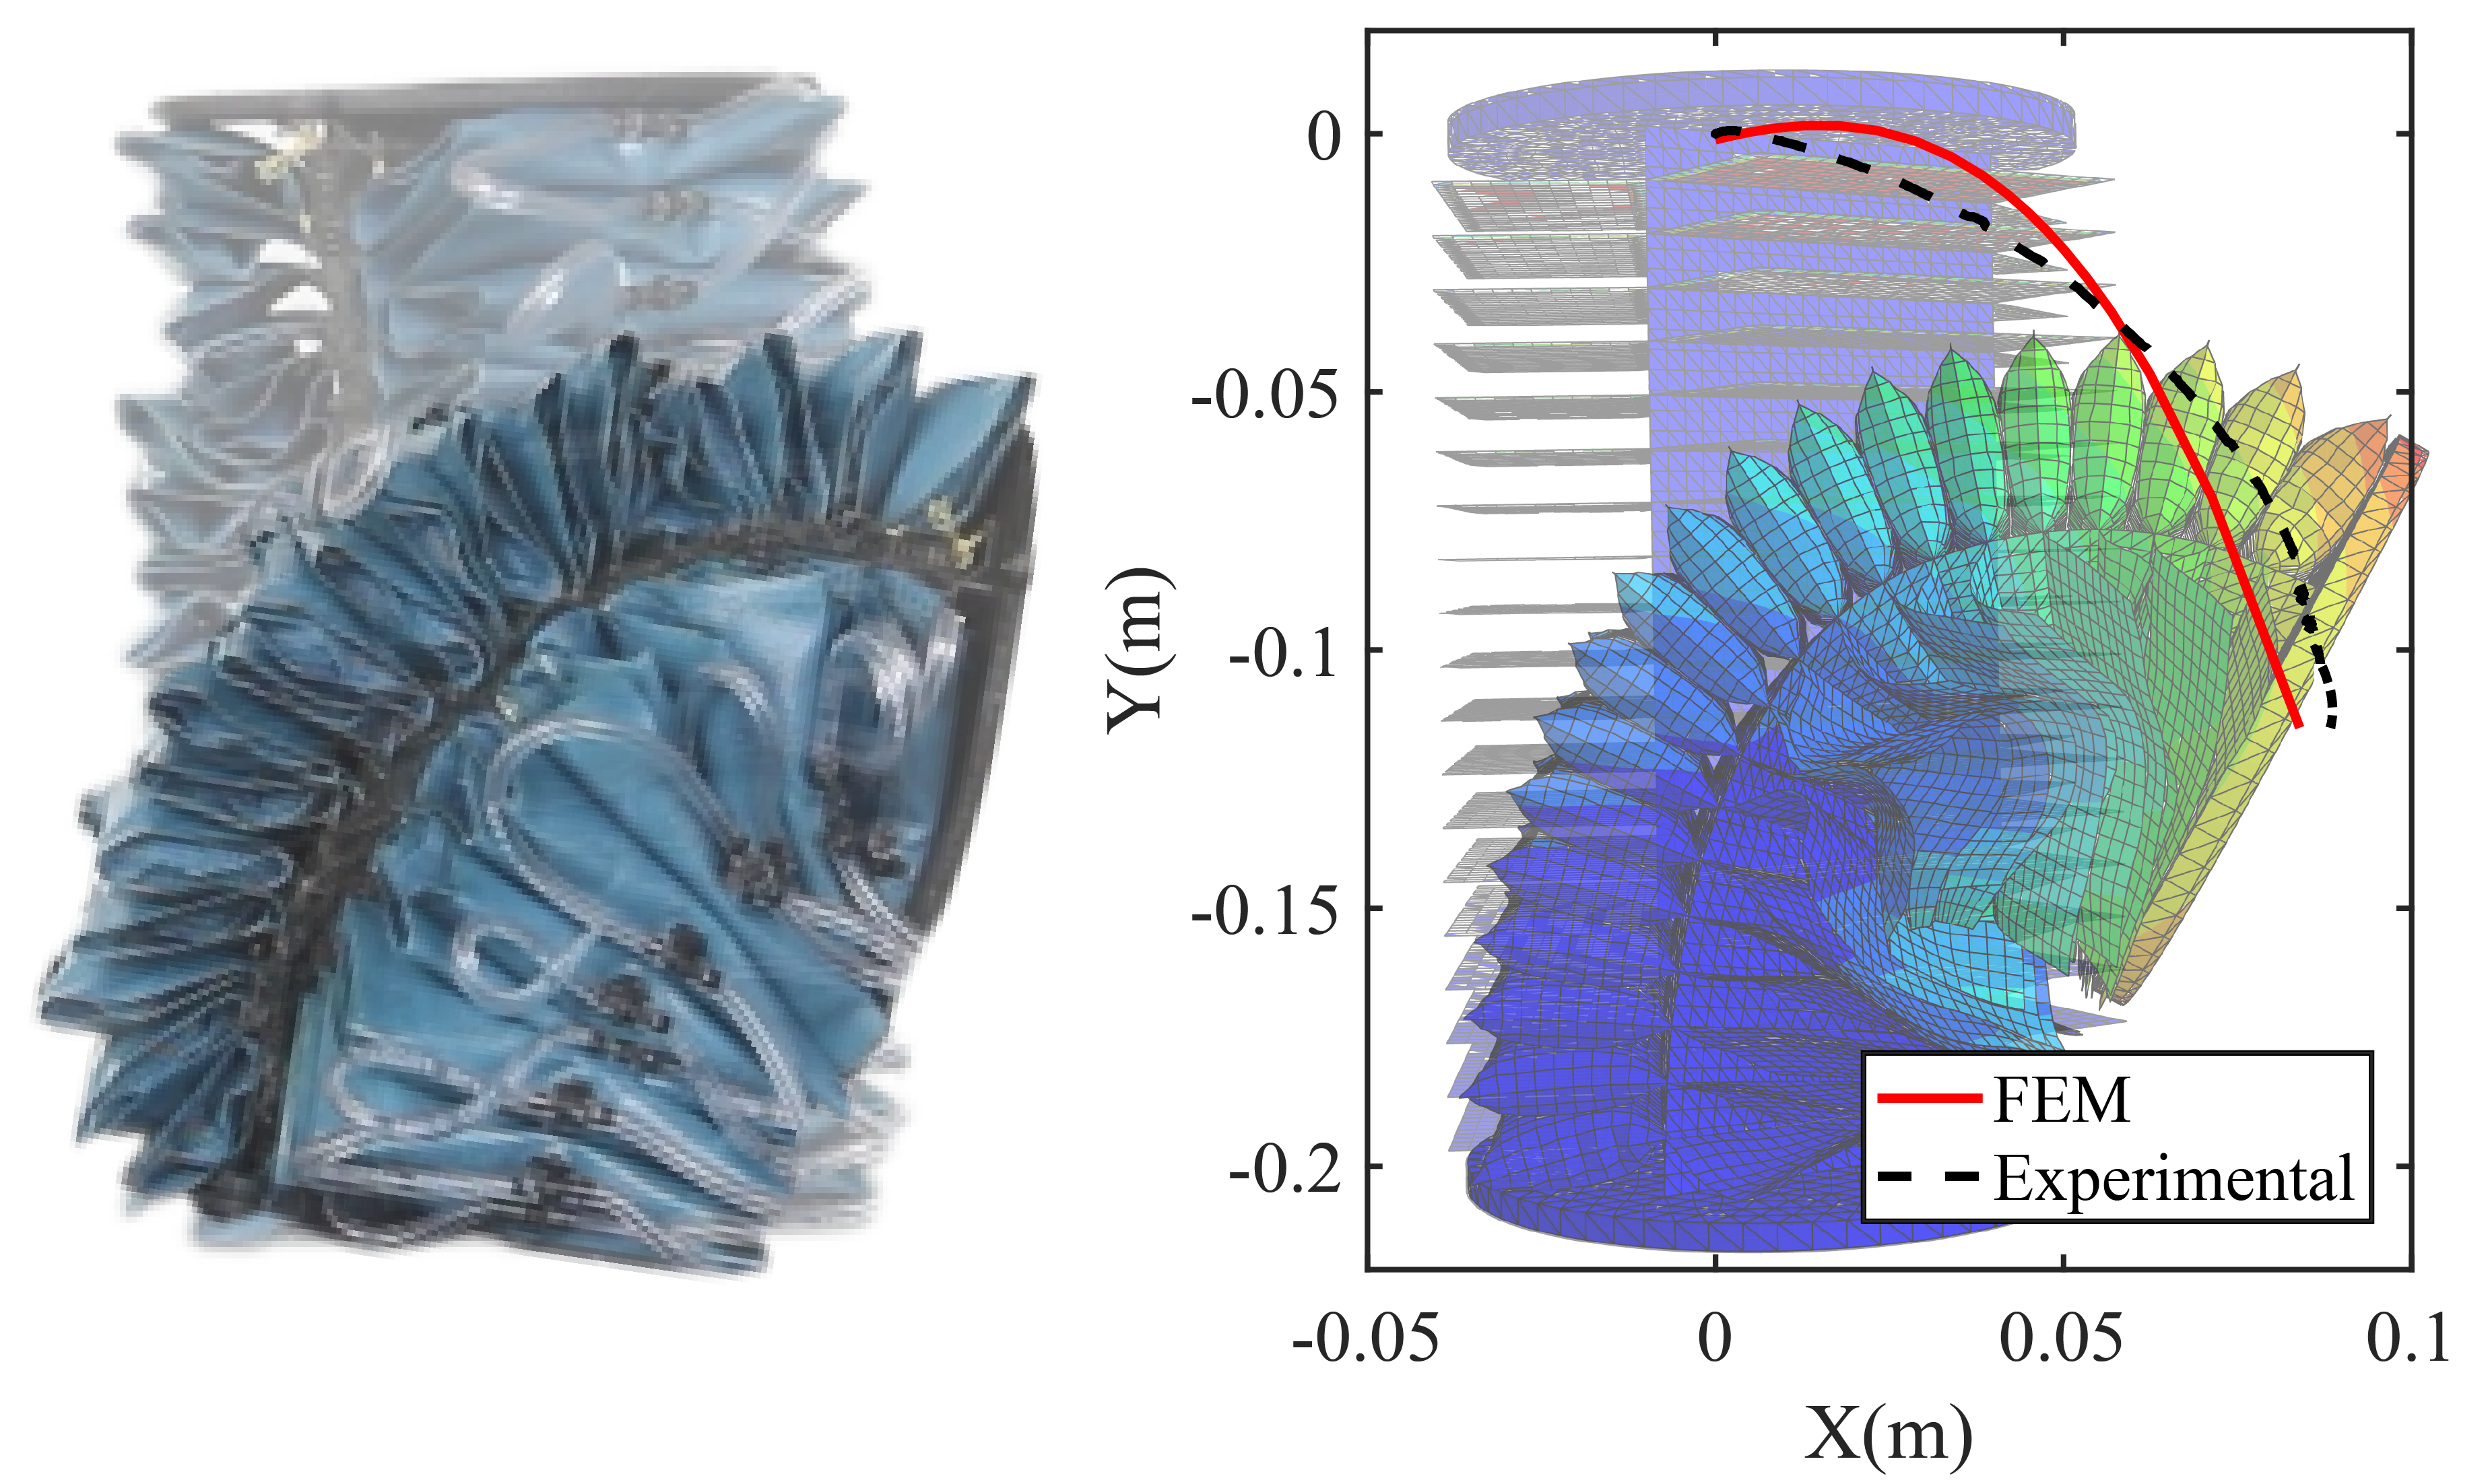
\includegraphics[width=0.48\textwidth]{Figures/fem_real_v4}
\caption{Bending Capability of a f3CBA unit compared between FEM and Experimentally Validated}
\label{fig:f3CAs_bend_fem_real}
\vspace{-1.5em}
\end{figure}


\begin{figure}[t!]
\centering
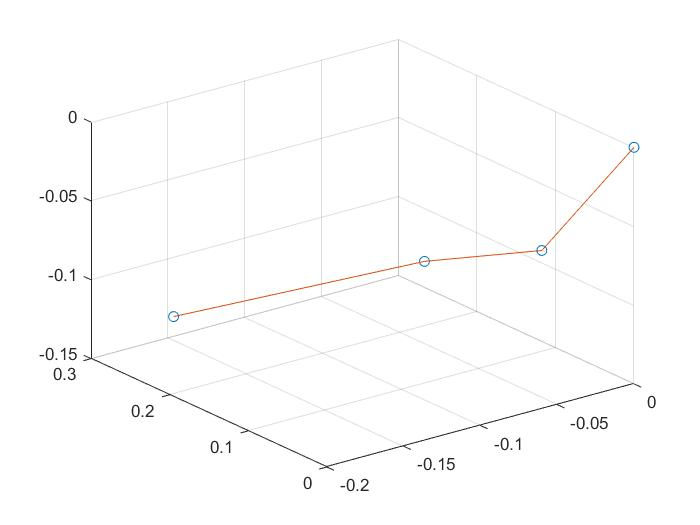
\includegraphics[width=0.45\textwidth]{Figures/SnakePose.jpg}
\caption{PLACEHOLDER Comparison of the FEM prediction of an arbitrary pose vs the resulting pose recorded via motion capture}
\label{fig:pose}
\end{figure}
\subsection{Payload Capacity}

To explore the payload capacity prior to fabricating the prototype, FEM models of the actuator array, f3CBA, and fSPL are developed and tested. The FEM models of the fSPL and its components are designed to inflate upwards against a force plate where the payload is measured at small pressure increments of  0.069$MPa$ until 0.34$MPa$ is reached. These models are then experimentally validated using a universal tensile testing machine (Instron 5944, Instron Corp., High Wycombe, United Kingdom) each in three repeated trials. Further, the free-space payload of f3CBA and fSPL, are tested by lifting loads from a deflated state. 
% * <polygerinos@asu.edu> 2018-09-10T01:00:59.766Z:
%
% > each in three repeated trials
%
% ^.
% * <polygerinos@asu.edu> 2018-09-10T01:00:09.655Z:
% 
% > 0.34$MPa$ 
% what that specific pressure sets the limit?explain
% 
% ^.

\subsubsection{Payload Capacity of the actuator array}
\label{sec:act_array_fem_real}

As seen in Fig. ~\ref{fig:opti_payload}a the actuator array is inflated upwards against the force plate of a UTM, constrained to push only in the vertical direction. Both FEM and experimental data demonstrated similar load output trends with a root mean square error (RMSE) of 9.087$N$. The single actuator array, weighing 0.098$kg$, is capable of producing 177.2$N$ in the FEM simulation and 174.7$\pm$6.367$N$, demonstrating a discrepancy error of 1.4\%. 


\subsubsection{Payload Capacity of the f3CBA}

For a single f3CBA segment, the load capacity when the two bottom adjacent actuator arrays were inflated, is evaluated in FEM and experimentally as seen in Fig. \ref{fig:opti_payload}b. Both the experimental and FEM simulation data when compared presented an RMSE of 4.057$N$. A result of 56.9$N$ and 53.7$\pm$1.041$N$ is shown for the FEM simulation and experimentally, respectively. that effectively corresponds to an error between the two of 5.62\%. 
% * <polygerinos@asu.edu> 2018-09-10T01:04:11.200Z:
% 
% > he two bottom adjacent actuator arrays were inflated
% what do you mean?
% 
% ^.

Furthermore, we test the free-space payload of a f3CBA, by fixing a single f3CBA segment in the horizontal direction and attaching weights at its distal end. The segment is pressurized until its body is parallel to the ground. The f3CBA is found capable of lifting a load of 5.5$kg$, approximately 15.1$x$ its own weight of 0.37$kg$.


\subsubsection{Payload Capacity of the fSPL}

Finally, the payload capacity of the complete fSPL is first predicted using the FEM model and then experimentally validated. The average load detected from the UTM force plate shows an average load of 14.91$\pm$0.926$N$, where the bottom adjacent chambers of the distal segments are pressurized up to 0.345$MPa$ and the bottom adjacent chambers in the proximal segment are pressurized up to 0.207$MPa$ to maintain the fSPL parallel the ground against gravity. The FEM model for the same setup demonstrates a payload of 20$N$, which deviates from the experimental by a 22.2\% error. 
% * <polygerinos@asu.edu> 2018-09-10T01:09:47.196Z:
% 
% > chambers
% know you call them chambers....similar to bladders...use a name throughout
% 
% ^.

Under the same pressurization scheme, weights are mounted at the proximal end of the fSPL and lifted to the position parallel against the ground. The maximum payload capacity of the 1.1$kg$ fSPL is found to be 1.5$kg$, surpassing the desired payload goal of 1$kg$ set in Section ~\ref{sec:func_req}.
% * <polygerinos@asu.edu> 2018-09-10T01:12:16.834Z:
% 
% > 1.1$kg$ fSPL
% i hope you are not including the base and pouch
% 
% ^.


\begin{figure}[b!]
\centering
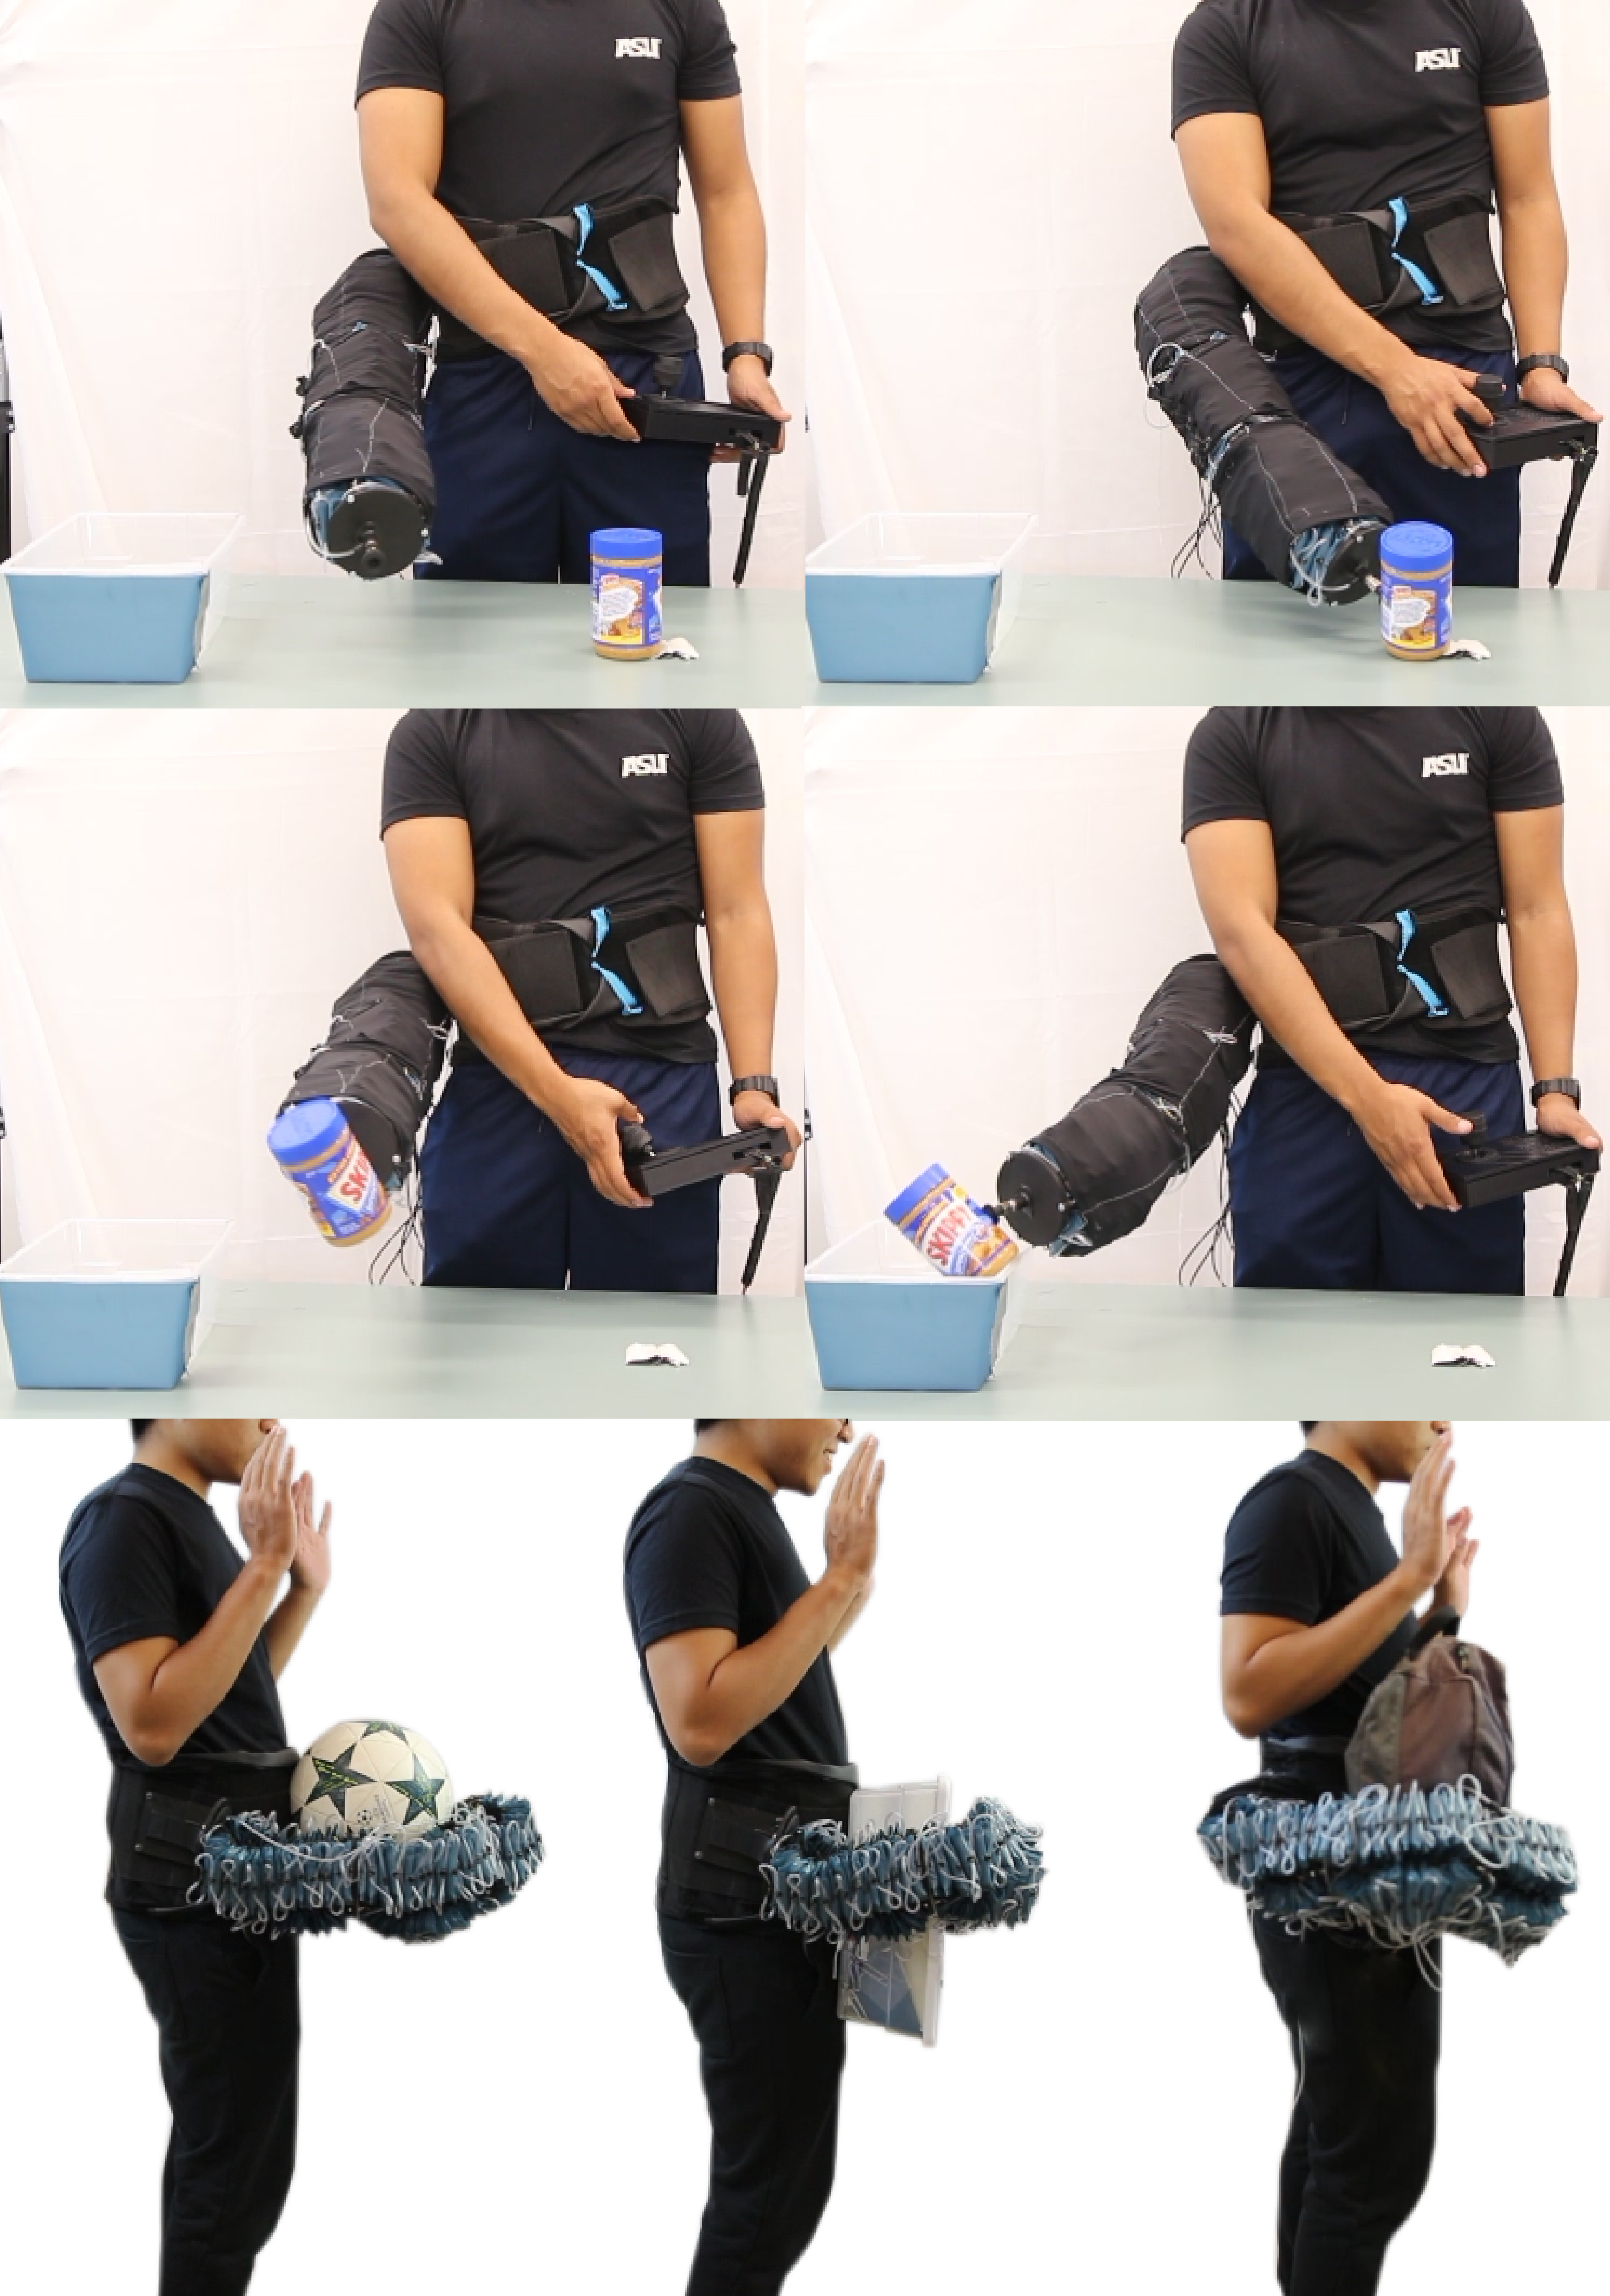
\includegraphics[width=0.45\textwidth]{Figures/pick_place_whole_body}
\caption{The different methods the fSPL can carry payload, either using its end-effector or whole body to wrap around objects.}
\label{fig:pick_place_whole_body}
\vspace{-1.5em}
\end{figure}


\subsection{FEM vs Experimental: Trajectory Tracking}

%Why are there two FEM vs Experimental sections here?
% \subsubsection{f3CBA FEM vs Experimental}
\subsubsection{f3CBA Motion Trajectory}

% \begin{figure}[b!]
% \centering
% 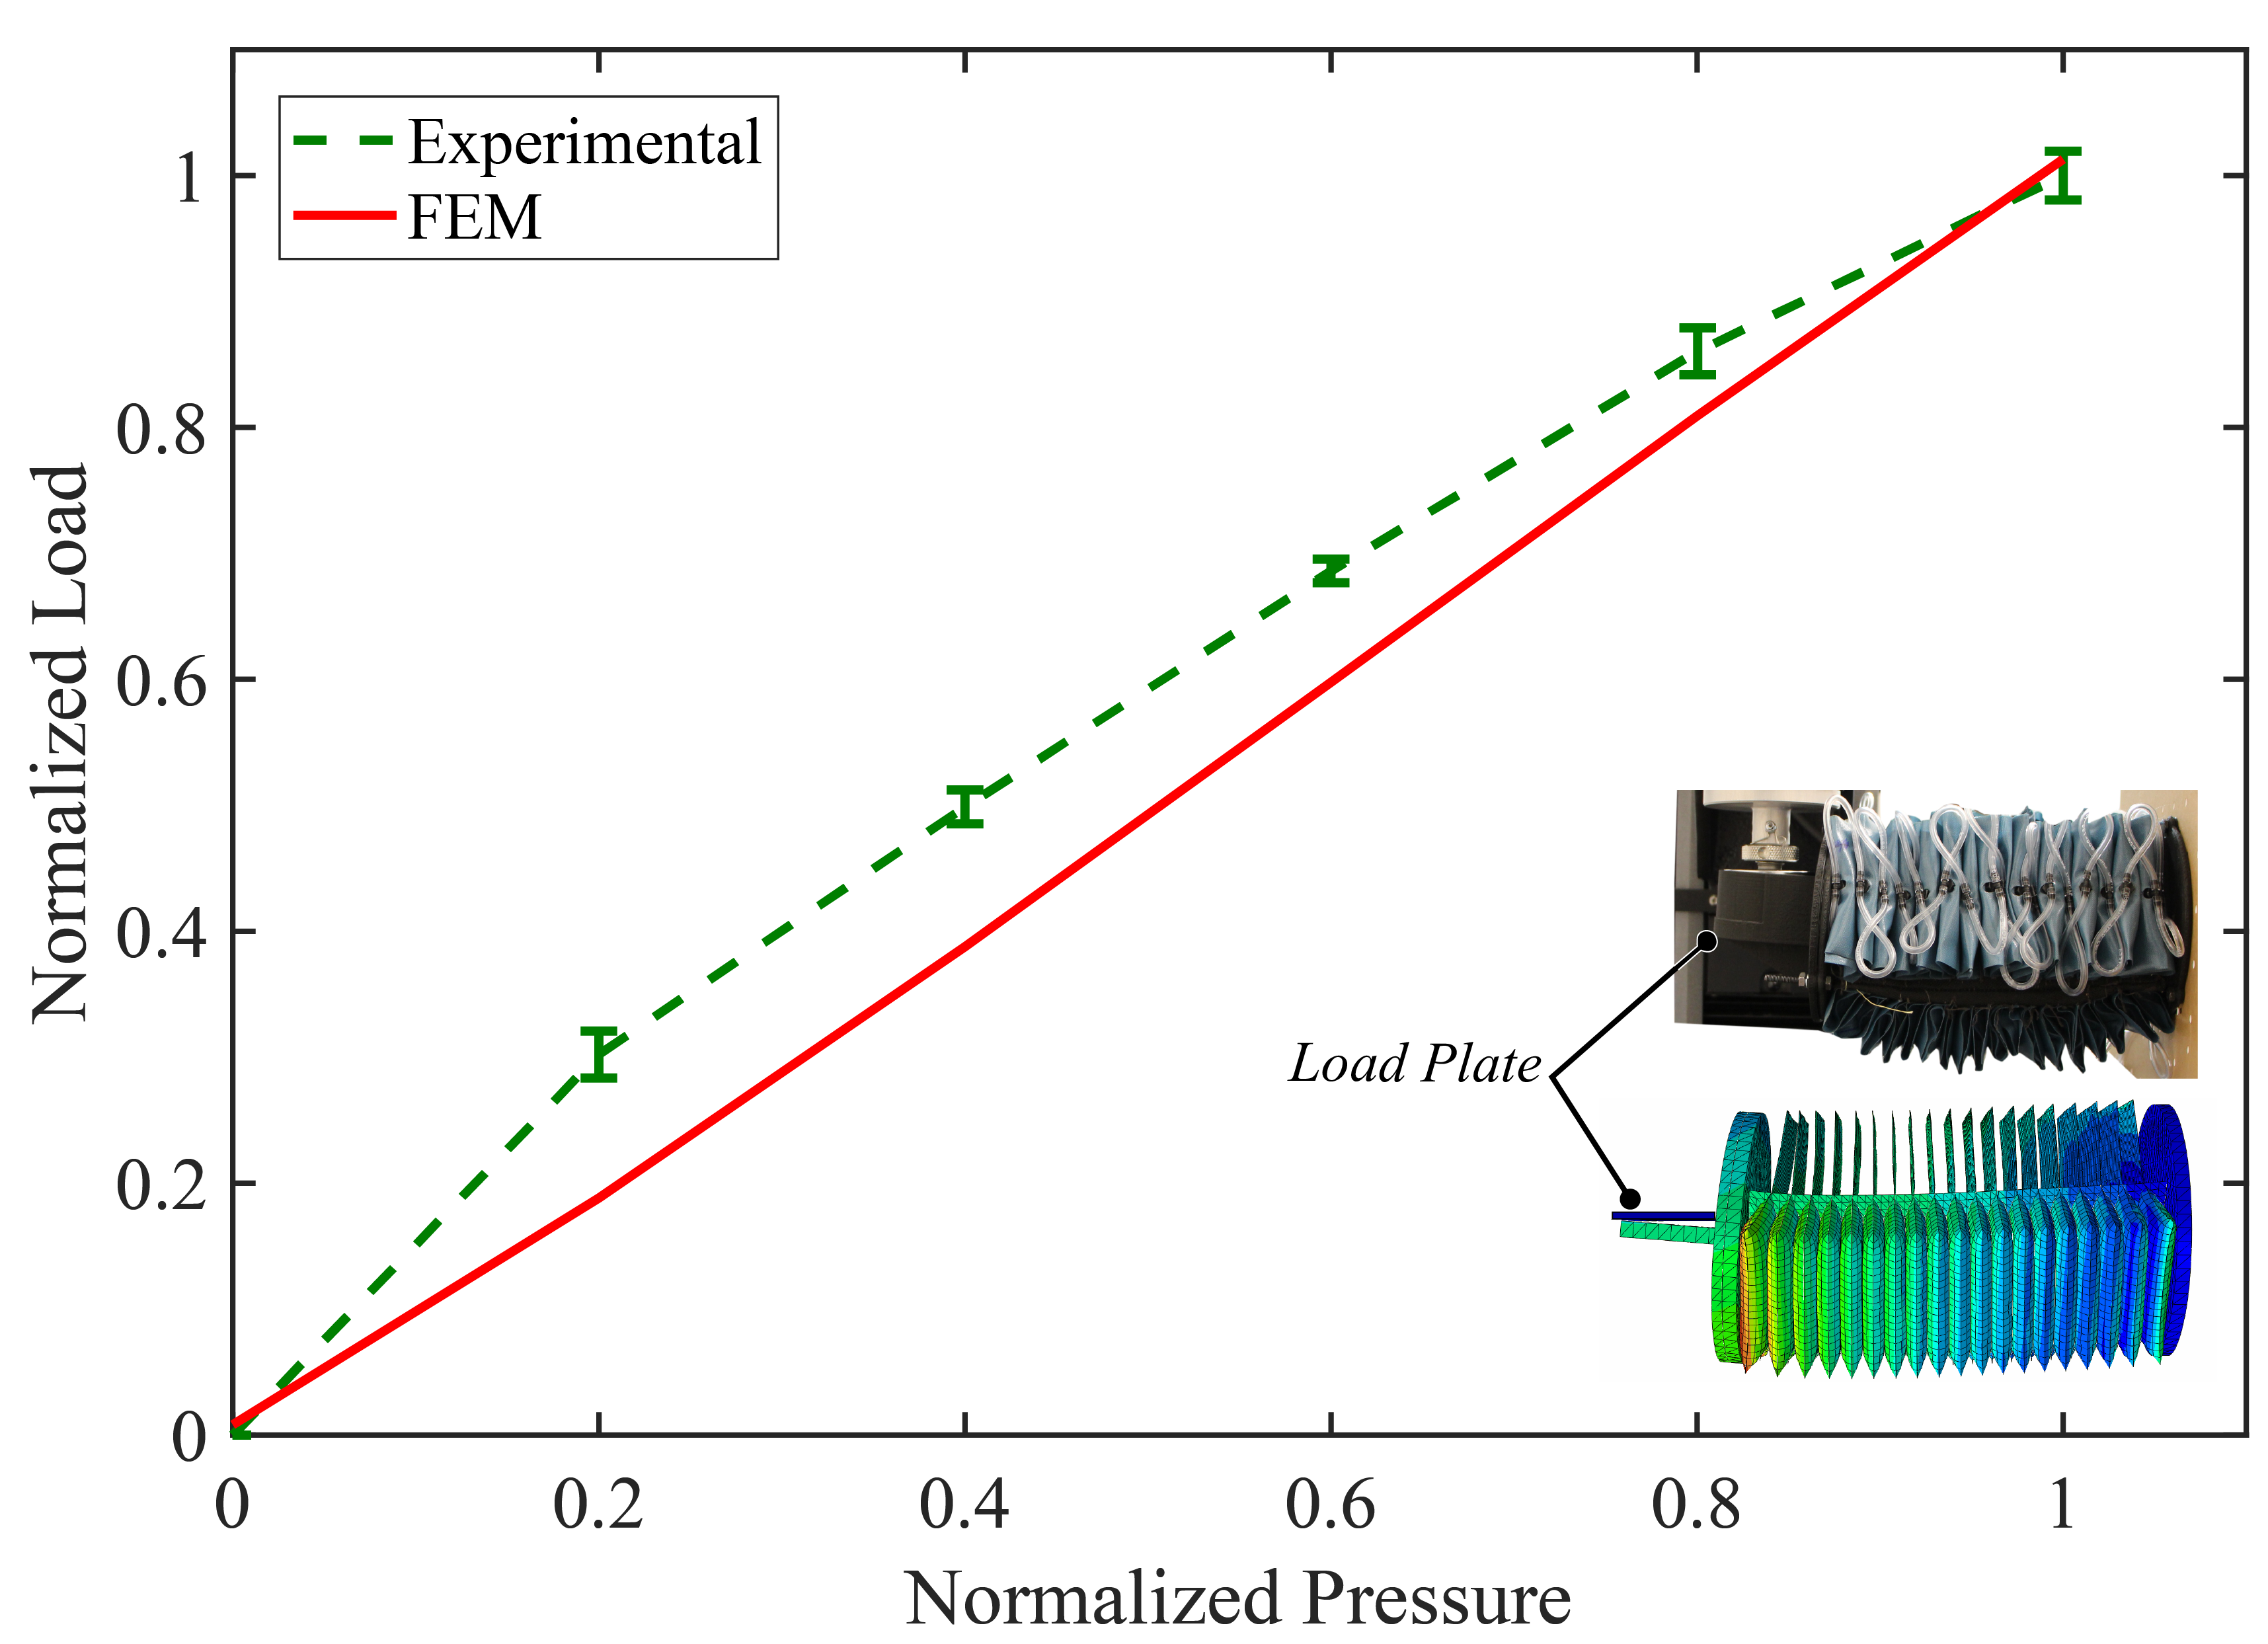
\includegraphics[width=0.45\textwidth]{Figures/3CA_instron}
% \caption{Payload Capability of a f3CBA unit compared between FEM and Experimentally Validated}
% \label{fig:f3CAs_load_fem_real}
% \vspace{-1.5em}
% \end{figure}




An experiment to compare the motion motion trajectory of a f3CBA segment of the FEM model with this of the prototype is conducted. A set of passive reflective markers are attached to the distal end of the segment to create a rigid body in the center of the distal enter and the motion capture system is used to track the motion of the distal end when one side of the segment is inflated up to 0.345$MPa$ in a quasi-static experiment, as seen in Fig. \ref{fig:f3CAs_bend_fem_real}. The distal end position of the 3CA in the FEM simulation and physical experiment results in a Euclidean distance error of 6.8$mm$. The rather close match between the trajectories of the model and experimental data shows that the FEM model can be used to predict the complex motion of a single segment of the fSPL.
% * <polygerinos@asu.edu> 2018-09-10T01:15:31.986Z:
% 
% > uclidean distance error of 6.8$mm$
% what does that mean in terms of % error?
% 
% ^.
% * <polygerinos@asu.edu> 2018-09-10T01:14:14.557Z:
% 
% > in the center of the distal enter 
% what are you trying to say here? revise
% 
% ^.


\subsubsection{fSPL Motion Trajectory}

We determine the FEM model to predict the continuum complex non-linear motion produced by the entire fSPL, a single complex pose is generated and recorded using the motion capture system. Four sets of motion markers are added at the proximal and distal end of every segment to create a virtual rigid body for the physical body of the fSPL. The fSPL is mounted perpendicular to the vector of gravity, and the lower two chambers of the first segment are inflated to 0.207$MPa$ and 0.345$MPa$ respectively, the lower right chamber of the second segment is subsequently inflated to 0.207$kPa$, and finally the lower left chamber of the third segment is inflated to 0.207$MPa$ to generate an arbitrary snake-like motion, as seen in Fig. \ref{fig:pose}. The experimental Euclidean displacement error is found to be \textbf{xxx} $mm$ when compared with the pose estimated by the FEM model. This adds to the conclusion that the FEM models created for the single bladder actuator array, the f3CBA, and the full fSPL can be good predictors of the load capability and complex motions generated by the interacting bladder actuator arrays.
% * <polygerinos@asu.edu> 2018-09-10T01:16:39.488Z:
% 
% > We determine the FEM model to predict the continuum complex non-linear motion produced by the entire fSPL, a single complex pose is generated and recorded using the motion capture system. 
% revise...not clear 
% 
% ^.




% \subsection{Payload Capacity of the fSPL}


% \begin{figure}[t!]
% \centering
% 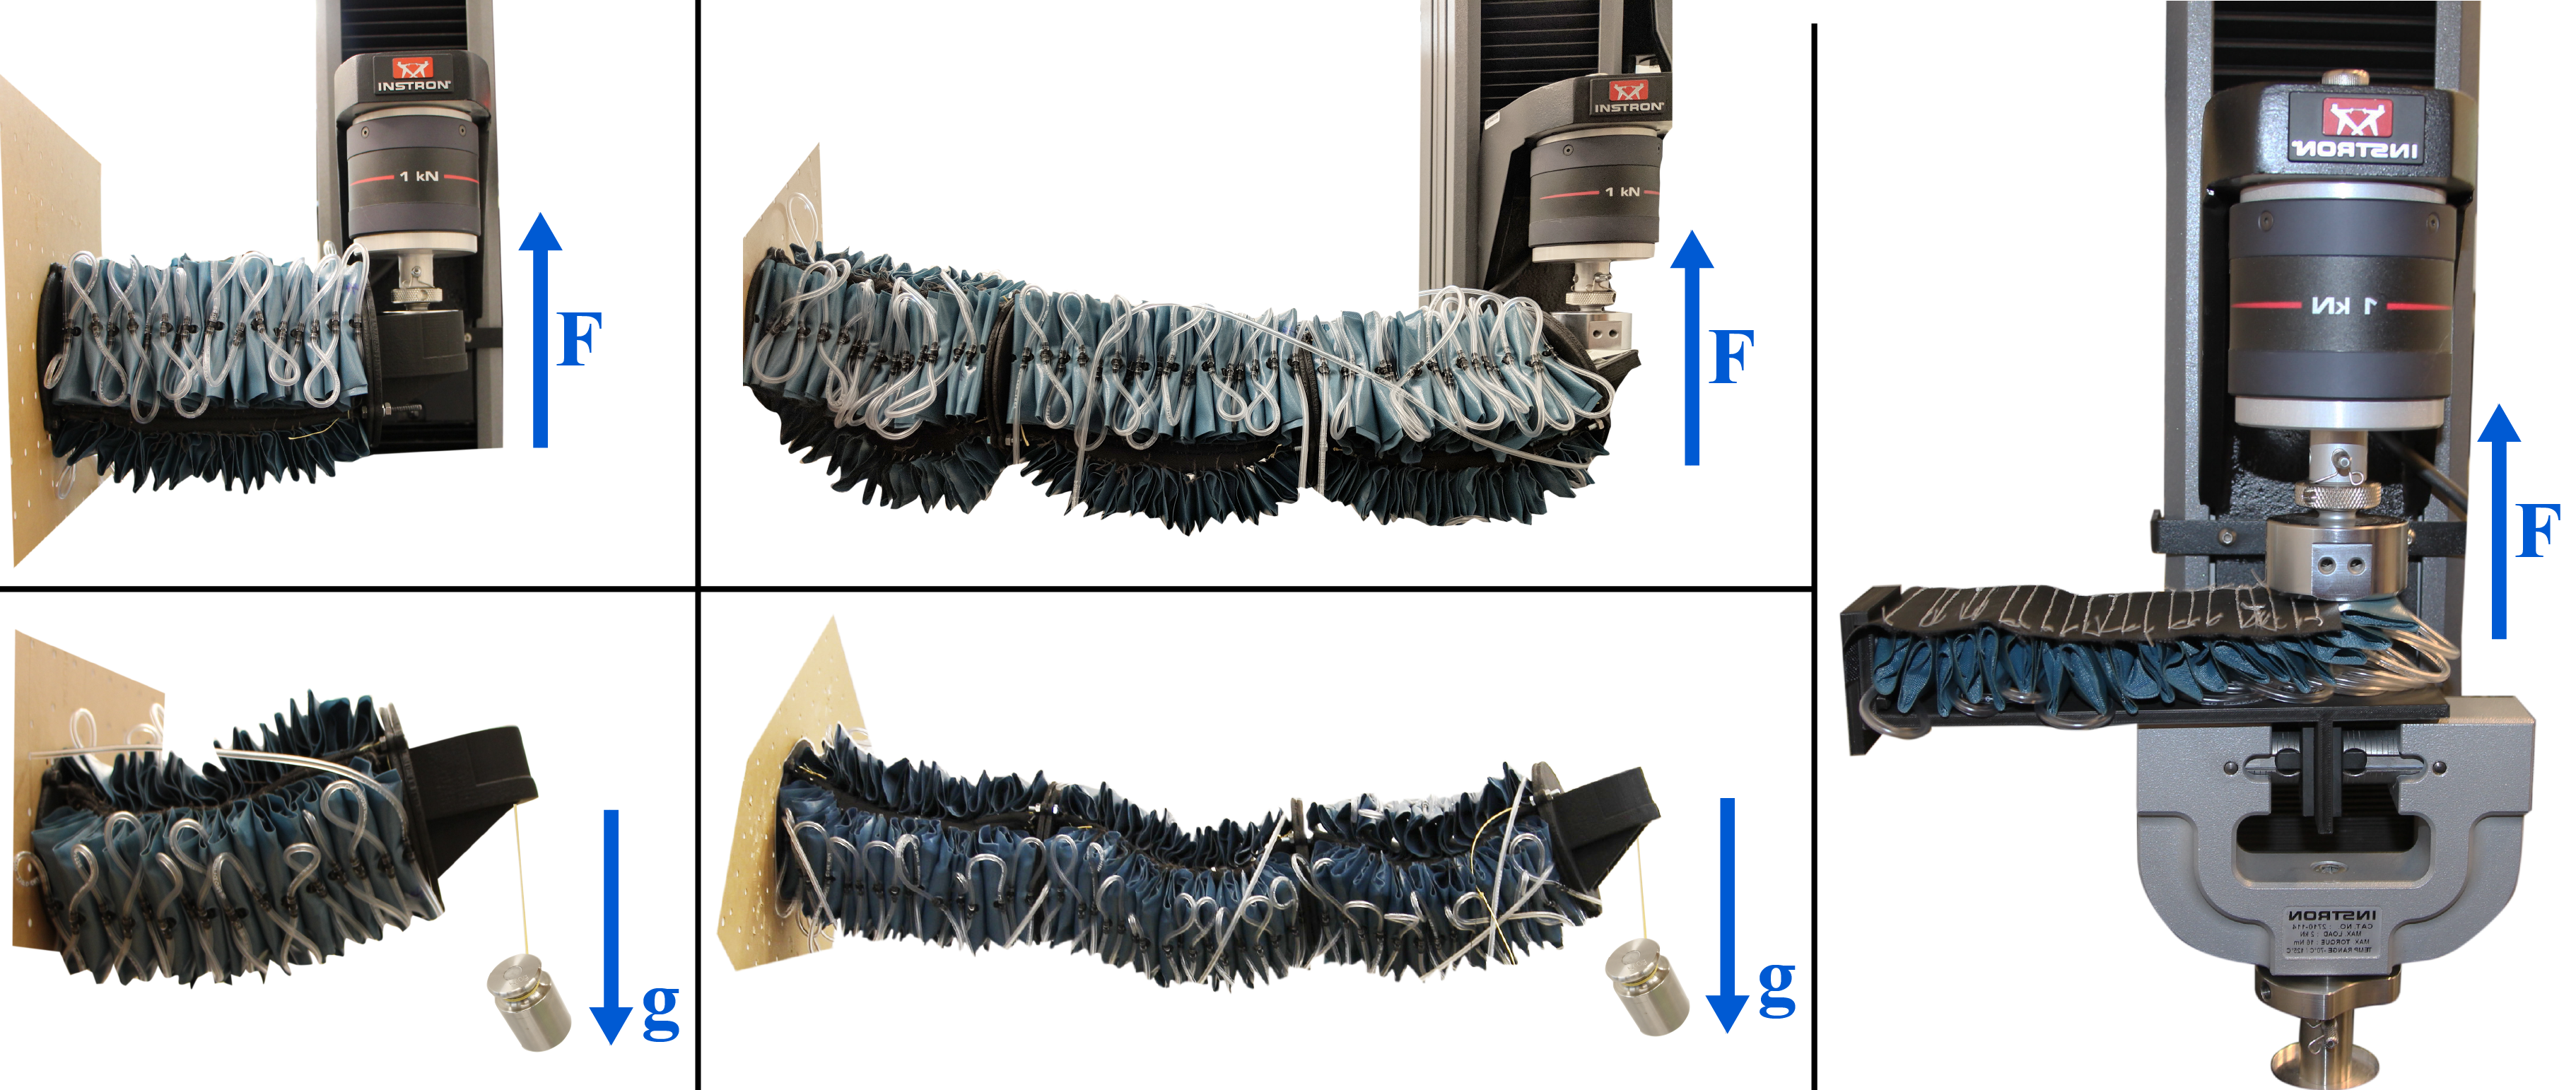
\includegraphics[width=0.45\textwidth]{Figures/payload_all_v2}
% \caption{Payload Setup for single bladder array, f3CBA, and fSPL}
% \label{fig:payload_all}
% \vspace{-1.5em}
% \end{figure}



\subsection{Pick and Place}


To test the effective fSPL payload, or the payload when the fSPL is used in real-life situation, along with user controllability, a pick-and-place experimental scheme is performed for multiple users. For this experiment, a vacuum suction cup is used at the fSPL's end-effector. The vacuum suction cup has a theoretical payload of 0.86$kg$ and is connected to a vacuum pump with depressurization rates of 1.42x10$^{-3}m^3/s$. The experiment is set up for the user to operate the fSPL using a joystick controller to, pick a jar with peanut butter (0.1$kg$) on one end of the table and move it across the table where a target box (0.33x0.16x0.12$m$) is placed 0.45$m$ away, as seen in Fig. \ref{fig:pick_place_whole_body}. Three users are timed while performing the task five times each.  User 1 improved their time from 53.28$s$ to 24.70$s$, user 2 improved from 45.34$s$ to 20.79$s$, and user 3 improved their time from 27.69$s$ to 17$s$. Thus preliminary demonstrating the gradual adoption and improvement in controlling a soft, external limb. A variety of other daily livings objects are also successfully picked and placed, including a canister of hair spray (0.43$kg$) and a water bottle 0.88$kg$.
% * <polygerinos@asu.edu> 2018-09-10T01:26:13.104Z:
% 
% > using a joystick controller to
% reviewers will ask about the controller...either reference past work or add a brief explanation here
% 
% ^.
% * <polygerinos@asu.edu> 2018-09-10T01:25:29.851Z:
% 
% > eir time from 53.28$s$ to 24.70$s$, user 2 improved from 45.34$s$ to 20.79$s$, and user 3 improved their time from 27.69$s$ to 17$s$. Thus preliminary demonstrating the gradual adoption and improvement in controlling a soft, external limb. A variety of other daily livings objects are also successfully picked and placed, including a canister of hair spray (0.43$kg$) and a water bottle 0.88$kg$.
% you need a table that shows all three objects and subsequent times performed in each trial for all users
% 
% ^.
% * <polygerinos@asu.edu> 2018-09-10T01:22:48.354Z:
% 
% >  for multiple users.
% how many?
% 
% ^.


% \subsubsection{Fold and Unfold}
% Our preliminary designs show that such compliant segment is able to linearly collapse two times its own length when squeezed, but also linearly deploy and perform multi-degree-of-freedom bending motions when pressurized (Figure 14).


% \begin{figure}[t!]
% \centering
% 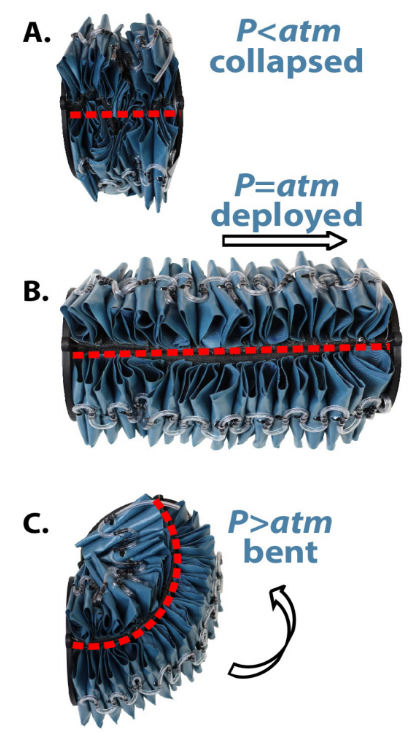
\includegraphics[width=0.30\textwidth]{Figures/unfold_fold}
% \caption{ Side view of soft fabric segment comprised of three bending
% soft fabric bundles in a triangle formation, able to collapse four 
% times its length and bend in multi-DoF when deployed and ressurized.}
% \label{fig:unfold_fold}
% \vspace{-1.5em}
% \end{figure}

\begin{figure}[t!]
\centering
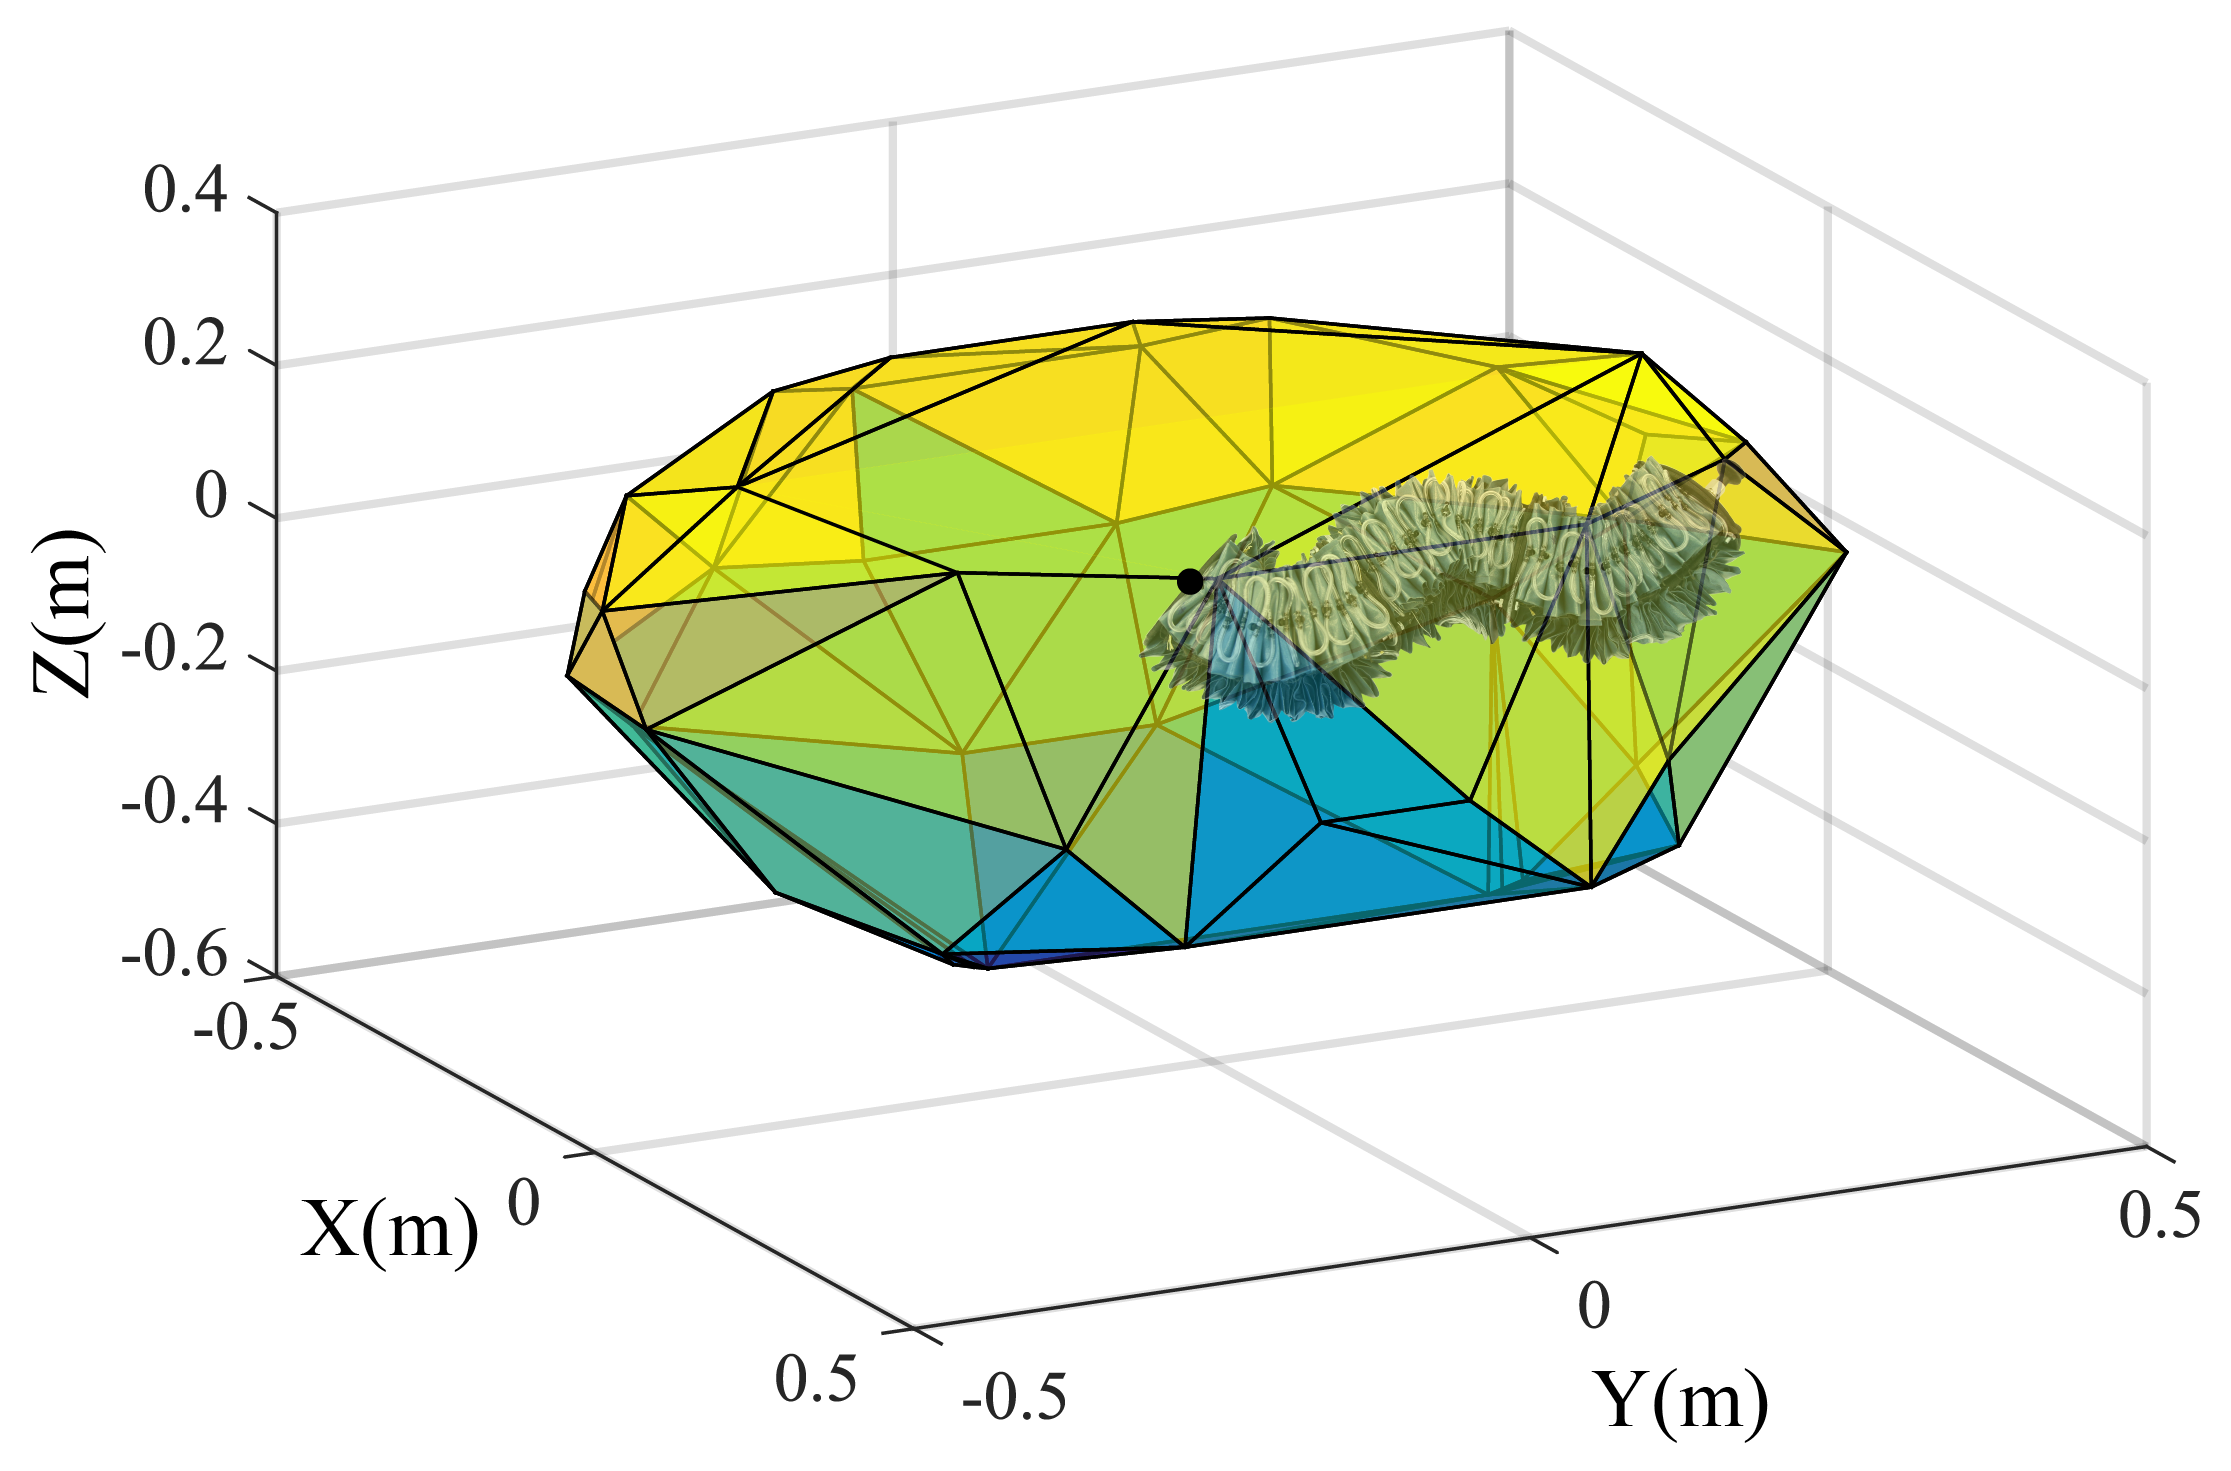
\includegraphics[width=0.45\textwidth]{Figures/Workspace_Fabric_ARM}
\caption{The different methods the fSPL can carry payload, either using its end-effector or whole body to wrap around objects.}
\label{fig:workspace_fabric_arm}
\vspace{-1.5em}
\end{figure}

\subsection{Whole-Body Continuum Grasping}

The fSPL is also capable of performing grasping by wrapping itself around objects, similar to how an elephant can grasp objects with its trunk. This method of grasping allows the fSPL to carry heavier and larger objects than capable by its end-effector. To demonstrate this unique feature the fSPL is attached to a belt worn by a user and is inflated to wrap around various objects. The objects tested includ a ball weighing 0.45$kg$, a box weighing 1.75$kg$, and a backpack weighing XXX, $kg$, as seen in Fig. \ref{fig:pick_place_whole_body}. The maximum payload capacity of the fSPL using the method is tested by gradually adding weights into the backpack resulting in a load of 4.51$kg$ (4.5$x$ its own body weight).


\subsection{Workspace}


To evaluate the effective workspace of the fSPL, the limb is mounted parallel to the ground, against gravity. Two sets of reflective markers are placed on the distal end and proximal end of the fSPL to create virtual rigid bodies. The individual chambers of the limb are inflated in various combinations up to an operating pressure of 0.34$MPa$ to cover its entire workspace. The position of the markers is recorded using a motion capture system with six cameras (Optitrack Prime 13W, NaturalPoint Inc., Corvallis, OR). The workspace of the fSPL is generated from the collected end-effector positions shown in Fig \ref{fig:workspace_fabric_arm}. The fSPL is shown capable of reaching any point inside the workspace and therefore the workspace volume of the fSPL is 0.22m$^{3}$, the maximum vertical range of the fSPL is 0.63$m$ and the maximum horizontal range of the limb is 0.65$m$. 
% * <polygerinos@asu.edu> 2018-09-10T01:30:40.090Z:
% 
% > he workspace volume of the fSPL is 0.22m$^{3}$, the maximum vertical range of the fSPL is 0.63$m$ and the maximum horizontal range of the limb is 0.65$m$. 
% Can you add a comment on what that means for a human operating range? what is human arms range?
% 
% ^.





% \begin{figure}[t!]
% \centering
% 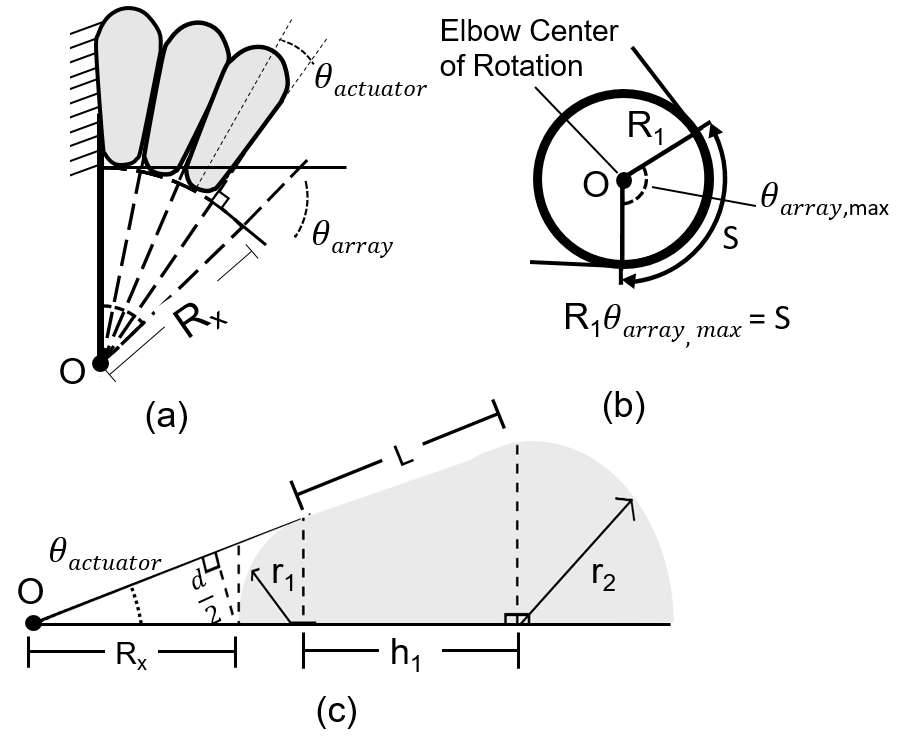
\includegraphics[width=0.45\textwidth]{model3.PNG}
% \caption{(a) Simple bladder arrangement demonstrating interactions in the array.  (b) Spherical elbow joint representation of constant radius. $S$. The length of the actuator array is defined with this model. (c) Section view of an individual actuator depicting dimensions used in calculating the interacting area. }
% \label{fig:hotness}
% \end{figure}
%\textcolor{red}{S=R1theta0 and theta1 is centerline to interacting edge }



% \begin{equation}\label{r1}
% 	r_1(\theta_{actuator})  = \frac{d}{2cos(\theta_{actuator})}.
% \end{equation}

% While the major radius, $r_2$, also utilizes the tangent, the solution is expressed as
%  \begin{equation}\label{r2}
% 	r_2(\theta_{actuator})  = -b + \sqrt{\frac{b^2-4ac}{2a}} ,
% \end{equation}
% where $a$, $b$, and $c$ are defined by

% \begin{equation}\label{a}
% 	a = 1+\frac{1}{(\pi R+\sqrt{(R_x+r_1)^2+r_1^2})^2}+(\frac{\pi}{2})^2 ,
% \end{equation}
% \begin{equation}\label{a}
% 	b = \pi^2R+\pi\sqrt{(R_x+r_1)^2+r_1^2}-\frac{\pi^2r_1}{2} ,
% \end{equation}
% \begin{equation}\label{a}
% \begin{aligned}
% \begin{multlined}
% 	c = (\pi R+\sqrt{(R_x+r_1)^2+r_1^2})^2- (\pi R+\lambda)^2...\\\\
%    +\pi^2Rr_1-(\frac{\pi R}{2})^2+\sqrt{(R_x+r_q)^2+r_1^2}\pi r_1 .
%     \end{multlined}
%     \end{aligned}
% \end{equation}



\section{Conclusion and Future Work}

In this paper, the design, development, and evaluation of a novel, user-mounted, Soft Poly-Limb (fSPL) is introduced utilizing for its operation high strength fabrics. The highly-articulated, soft fSPL is designed towards supporting and assisting in the future impaired individuals. The fSPL’s geometrical parameters are initially optimized and experimentally validated using quasi-static computational FEM models providing design guidelines for the community to design fSPLs based on the desired payload capacity and articulation performance.

Each fSPL segment was capable of effectively lifting 15.1 times its own weight at 5.5$kg$ and the fSPL was also able to carry up to 1.5$kg$ while still being able to maneuver in space in various pick-and-place experiments holding daily living objects. By employing the whole body grasping strategy, the fSPL could wrap and carry loads of up to 4.5$kg$, over 4 times it’s own body weight.

The fSPL was shown to be capable of safely operating around a user with a large workspace and be able to safely interact with the environment. The fSPL’s modular design also allowed the rapid swapping of actuators and interchangeable segments, if maintenance is required. 

Future work will introduce the exploration of multi-mounting positions and multiple interacting fSPLs on one user to expand the user’s workspace and capabilities of controlling multi-external limbs. Further exploration of various hands-free user-intent detection methods will also be explored. Implementation of a decentralized and distributed on-board actuation and power supply systems that are capable of controlling such a complicated system is being explored. Future efforts are being made to control the SPL using distributed sensing and control methods \cite{Wenlong2018} with the exploration of soft-distributed and embedded sensing technologies as well. 
% * <polygerinos@asu.edu> 2018-09-10T01:37:21.810Z:
% 
% > Implementation of a decentralized and distributed on-board actuation and power supply systems that are capable of controlling such a complicated system is being explored. Future efforts are being made to control the SPL using distributed sensing and control methods \cite{Wenlong2018} with the exploration of soft-distributed and embedded sensing technologies as well. 
% these two statements sounds a bit repetitive with one another..please revise
% 
% ^.

% In total, we believe that this work provides the readers with the capability of designing highly lightweight and soft robotic limbs capable of being easily stored and deployed on-site capable of support the versatile amount of activities of daily living.




%%%%%%%%%%%%%%%%%%%%%%%%%%%%%%%%%%%%%%%%%%%%%%%%%%%%%%%%%%%%%%%%%%%%%%%%%%%%%%%%

\section*{ACKNOWLEDGMENTS} 
This work was supported in part by the National Science Foundation under Grant CMMI-1800940.

%%%%%%%%%%%%%%%%%%%%%%%%%%%%%%%%%%%%%%%%%%%%%%%%%%%%%%%%%%%%%%%%%%%%%%%%%%%%%%%%



%%%%%%%%%%%%%%%%%%%%%%%%%%%%%%%%%%%%%%%%%%%%%%%%%%%%%%%%%%%%%%%%%%%%%%%%%%%%%%%%
%%%%%%%%%%%%%%%%%%%%%%%%%%%%%%%%%%%%%%%%%%%%%%%%%%%%%%%%%%%%%%%%%%%%%%%%%%%%%%%%


% ********************************** Bibliography ******************************
\bibliographystyle{unsrt}
%\bibliographystyle{plain}
%\bibliographystyle{plainnat} % use this to have URLs listed in References
%\cleardoublepage
\bibliography{ICRA2019.bib} % Path to your References.bib file



% \begin{thebibliography}{99}
% * <polygerinos@asu.edu> 2018-09-10T01:38:13.690Z:
% 
% > % \begin{thebibliography}{99}
% you bibliography has wrong format...it should be P. Polygerinos not Panagiotis Polygerinos that is now...
% 
% ^.
% \bibitem{c1} G. O. Young, ÒSynthetic structure of industrial plastics (Book style with paper title and editor),Ó 	in Plastics, 2nd ed. vol. 3, J. Peters, Ed.  New York: McGraw-Hill, 1964, pp. 15Ð64.
% \bibitem{c2} W.-K. Chen, Linear Networks and Systems (Book style).	Belmont, CA: Wadsworth, 1993, pp. 123Ð135.
% \bibitem{c3} H. Poor, An Introduction to Signal Detection and Estimation.   New York: Springer-Verlag, 1985, ch. 4.
% \bibitem{c4} B. Smith, ÒAn approach to graphs of linear forms (Unpublished work style),Ó unpublished.
% \bibitem{c5} E. H. Miller, ÒA note on reflector arrays (Periodical styleÑAccepted for publication),Ó IEEE Trans. Antennas Propagat., to be publised.
% \bibitem{c6} J. Wang, ÒFundamentals of erbium-doped fiber amplifiers arrays (Periodical styleÑSubmitted for publication),Ó IEEE J. Quantum Electron., submitted for publication.
% \bibitem{c7} C. J. Kaufman, Rocky Mountain Research Lab., Boulder, CO, private communication, May 1995.
% \bibitem{c8} Y. Yorozu, M. Hirano, K. Oka, and Y. Tagawa, ÒElectron spectroscopy studies on magneto-optical media and plastic substrate interfaces(Translation Journals style),Ó IEEE Transl. J. Magn.Jpn., vol. 2, Aug. 1987, pp. 740Ð741 [Dig. 9th Annu. Conf. Magnetics Japan, 1982, p. 301].
% \bibitem{c9} M. Young, The Techincal Writers Handbook.  Mill Valley, CA: University Science, 1989.
% \bibitem{c10} J. U. Duncombe, ÒInfrared navigationÑPart I: An assessment of feasibility (Periodical style),Ó IEEE Trans. Electron Devices, vol. ED-11, pp. 34Ð39, Jan. 1959.
% \bibitem{c11} S. Chen, B. Mulgrew, and P. M. Grant, ÒA clustering technique for digital communications channel equalization using radial basis function networks,Ó IEEE Trans. Neural Networks, vol. 4, pp. 570Ð578, July 1993.
% \bibitem{c12} R. W. Lucky, ÒAutomatic equalization for digital communication,Ó Bell Syst. Tech. J., vol. 44, no. 4, pp. 547Ð588, Apr. 1965.
% \bibitem{c13} S. P. Bingulac, ÒOn the compatibility of adaptive controllers (Published Conference Proceedings style),Ó in Proc. 4th Annu. Allerton Conf. Circuits and Systems Theory, New York, 1994, pp. 8Ð16.
% \bibitem{c14} G. R. Faulhaber, ÒDesign of service systems with priority reservation,Ó in Conf. Rec. 1995 IEEE Int. Conf. Communications, pp. 3Ð8.
% \bibitem{c15} W. D. Doyle, ÒMagnetization reversal in films with biaxial anisotropy,Ó in 1987 Proc. INTERMAG Conf., pp. 2.2-1Ð2.2-6.
% \bibitem{c16} G. W. Juette and L. E. Zeffanella, ÒRadio noise currents n short sections on bundle conductors (Presented Conference Paper style),Ó presented at the IEEE Summer power Meeting, Dallas, TX, June 22Ð27, 1990, Paper 90 SM 690-0 PWRS.
% \bibitem{c17} J. G. Kreifeldt, ÒAn analysis of surface-detected EMG as an amplitude-modulated noise,Ó presented at the 1989 Int. Conf. Medicine and Biological Engineering, Chicago, IL.
% \bibitem{c18} J. Williams, ÒNarrow-band analyzer (Thesis or Dissertation style),Ó Ph.D. dissertation, Dept. Elect. Eng., Harvard Univ., Cambridge, MA, 1993. 
% \bibitem{c19} N. Kawasaki, ÒParametric study of thermal and chemical nonequilibrium nozzle flow,Ó M.S. thesis, Dept. Electron. Eng., Osaka Univ., Osaka, Japan, 1993.
% \bibitem{c20} J. P. Wilkinson, ÒNonlinear resonant circuit devices (Patent style),Ó U.S. Patent 3 624 12, July 16, 1990.
% \end{thebibliography}




\end{document}
